\section{Stochastic Inference of Surface-Induced Effects Using Brownian Motion}

\subsection{Confined Brownian motion theory}

By observing the experimental trajectory along the $z$-axis of a particle of $1.5 ~ \mathrm{\mu m} $ radius as shown in Fig.~\ref{Fig:exp_z_traj}, one can notice that the particle's height does not get higher than approximately $4 ~ \mathrm{\mu m}$. Indeed, due to gravity, a colloid is confined near the surface. This confinement induces near-wall effects, such as hindered mobility and electrostatic interactions. 

In the first part of this chapter, I will detail the theory of confined Brownian motion and how to numerically simulate it. In a second part, I will present how to analyze experimental data. In particular, I will detail a multi-fitting procedure that a enables thermal-noise-limited inference of diffusion coefficients spatially resolved at the nanoscale, equilibrium potentials, and forces at the femtonewton resolution.

\begin{figure}[ht]
	\centering
	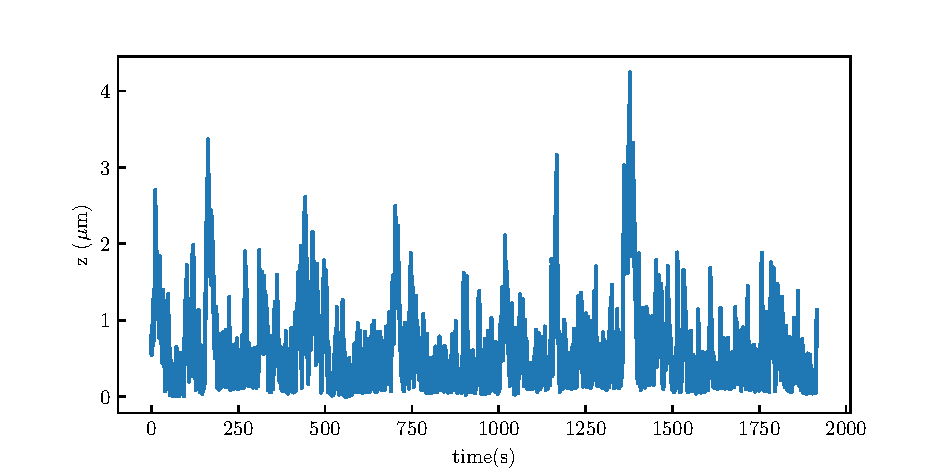
\includegraphics{02_body/chapter3/images/traj_z/traj_z.pdf}
	\caption{Experimental trajectory of a polystyrene particle of radius $a = 1.5 ~ \mathrm{\mu m}$ in water near a glass wall ($z = 0$) along the $z$-axis --- \textit{i.e} perpendicular to the wall.}
	\label{Fig:exp_z_traj}
\end{figure}

\subsubsection{Gravitational potential}


The density $\rho_\mathrm{p}$ of an observed colloid is different from the medium density $\rho_\mathrm{m}$. In our experiment, we used water whose density is $\rho_\mathrm{m} = 1000 ~ \mathrm{kg.m^{-3}}$. Thus, the particles are subject to gravitational potential given by:

\begin{equation}
	U_\mathrm{g} (z) = \Delta m g z = \frac{4}{3}\pi a ^3 g \Delta \rho z ~,
	\label{eq:ug_full}
\end{equation}

where $\Delta m$ is the difference between the mass of the particle and that of a fluid sphere of the same size, $\Delta \rho = \rho_\mathrm{m} - \rho_\mathrm{p}$ is the corresponding density difference, and $g$ is the gravitational acceleration. By invoking the definition of the Boltzmann length:

\begin{equation}
	\ell _\mathrm{B} = \frac{k_\mathrm{B}T}{(4/3) \pi a ^3 \Delta \rho g } ~,
\end{equation}

one can rewrite Eq.~(\ref{eq:ug_full}) as:

\begin{equation}
	U_\mathrm{g}(z) = \frac{k_\mathrm{B}T}{\ell _\mathrm{B}}z ~.
	\label{eq:ug}
\end{equation}

The Boltzmann length $\ell_\mathrm{B}$ corresponds to the spatial extent over which the change of gravitational energy equals thermal energy. This distance was first measured by Perrin \cite{perrin_les_2014}. To do so, using a microscope he counted the number of colloidal particles as a function of the height in the sample. Then, he reconstructed the concentration profile of the colloidal suspension that exponentially decays as $\mathrm{e}^{- z / \ell _\mathrm{B}}$. As an example, for a polystyrene particle of radius $a  = 1.5 ~ \mathrm{\mu m}$ in water, one has $\ell _\mathrm{B} = 580 ~ \mathrm{nm}$.

For systems with $\ell _\mathrm{B} >> h $, whiere $h$ is the vertical thickness of the sample, one can consider that the particle does not feel gravity. This is particularly the case when the densities of the colloids and the fluid are equal. In this particular case, one has $\ell _\mathrm{B} = \infty$. Thus, density matching can be a way to do gravitaty-free experiments. In our experiment, we want to measure confinement-induced effects. Therefore, we need gravity for particles to be driven towards the substrate. As particles get larger or denser, $\ell _\mathrm{B}$ decreases and particles are, on average, closer to the substrate. 


\subsubsection{Sphere-wall interactions}
\label{Section:sphere-wall}



As we have seen, external forces such as gravity act on the particles. As Brownian particles are close to a wall, we can also expect some interactions between the particles and the wall. In our case, we suppose that the Brownian particles do not interact with each other, as we consider dilute soultions only. Indeed, the studied particles are at least $50 ~ \mathrm{\mu m}$ apart from each other, which corresponds to 10 times their size for the largest beads. 

To describe the interaction between a Brownian particle and the wall, we use the DLVO theory, named after Derjaguin, Landau, Verwey, and Overbeek \cite{israelachvili_intermolecular_2015}. This theory was first developed to describe the interactions between colloids, and explains the stability of colloidal suspensions. It involves two force components; the Hamaker force which arises from van der Waals interactions between the molecules of the two surfaces and a screened electrostatic force due to a double layer of charges formed near each surface, and involving the ions present in the solution. 

\paragraph{Double layer interactions}\mbox{}\\
\vspace{0.10cm}


When a surface is immersed in water, it usually acquire charges \cite{israelachvili_intermolecular_2015} due to a high water dielectric constant $\epsilon = \epsilon_0 \epsilon_\mathrm{r}$, where $\epsilon_0$ is the vacuum permittivity and $\epsilon_\mathrm{r}$ the medium relative permittivity; for water $\epsilon_\mathrm{r} = 80$. Commonly, surface charging is done through the ionization of  surface groups\footnote{For example, the dissociation of protons from surface carboxylic groups \cite{israelachvili_intermolecular_2015} ($-$COOH $\rightarrow$ -COO$^-$ + H$^+$) which charges negatively the surface.}, or from the binding of ions from the solution --- for example, adsorption of $-$OH$^-$ onto the water-air interface that charges it negatively. In the bulk, a fluid is electrically neutral; thus the fluid contains as equal number of ions of opposite charges (including the proper stoichiometry due to ionic valencies). However, when a surface is negatively charged, the negative ions are repelled from it, while positive ions are attracted towards it.  Therefore, a double-layer charge distribution is formed near the surface, as shown in Fig.~\ref{Fig:double_layer}. Experimentally, we use glass slides and polystyrene beads that are both negatively charged in water leading to a repulsive interaction between them. This repulsive force prevents the colloids from sticking together, or to the substrate's surface.

The DLVO theory state that the electrostatic potential $\Psi(\vec{r})$ generated by an ion of one given speicies $i$ at a distance $\vec{r}$ satisfies the Poisson equation \cite{israelachvili_intermolecular_2015}:

\begin{equation}
	\nabla ^2 \Psi(\vec{r}) = -\frac{1}{\epsilon_\mathrm{r} \epsilon_0}  \rho_\mathrm{e}(\vec{r})~,
	\label{Eq:poisson}
\end{equation}

with:

\begin{equation}
	\rho_\mathrm{e}(\vec{r}) = e \sum _i z_i c_i (\vec{r}) ~,
	\label{Eq.3}
\end{equation}

\begin{figure}
	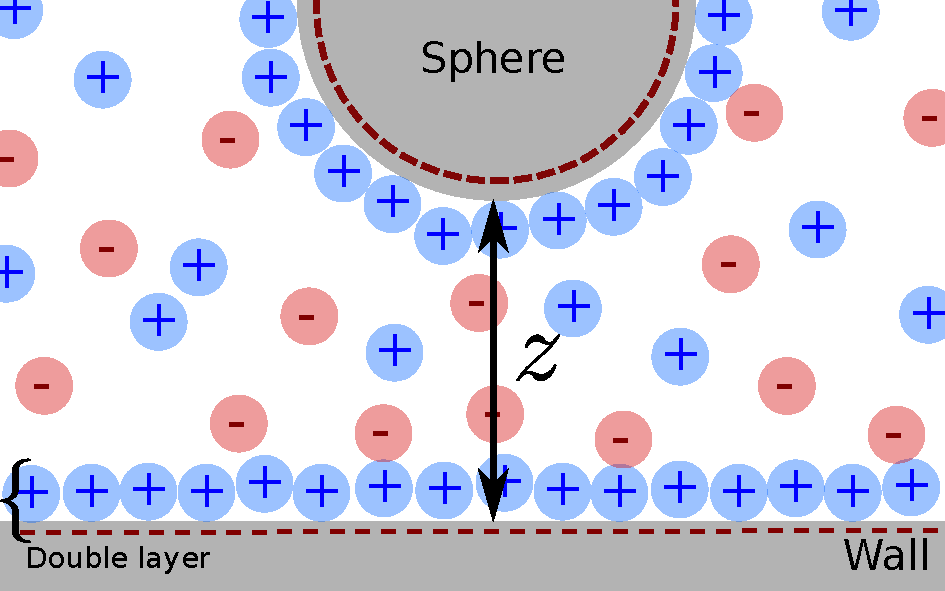
\includegraphics{02_body/chapter3/images/double_layer.pdf}
	\caption{A colloid diffusing near a wall. Both the wall and colloid surfaces charge negatively. As a consequence, a layer of positively-charged ions is attracted towards each surface, forming a double layer.}
	\label{Fig:double_layer}
\end{figure}


the local charge density, where $e$ is the elementary charge, and where the index $i$ denotes an ionic species of valence $z_i$ and local ionic concentration $c_i$ (number density). If the solution is at thermodynamic equilibrium, the local ionnic density is given by a Gibbs-Boltzmann distribution, as:

\begin{equation}
	c_i(\vec{r}) = c_i ^0 \textnormal{exp}\left(\frac{-z_i e \Psi(\vec{r})}{k_\mathrm{B} T }\right) ~,
	\label{Eq.4}
\end{equation}


where $c_i ^0$ is the bulk concentration (number density) of the ionic species $i$. By combining Eqs.~(\ref{Eq:poisson}),~(\ref{Eq.3})~and~(\ref{Eq.4}), one obtains the Poisson-Boltzmann equation:

\begin{equation}
	\nabla ^2 \Psi (\vec{r}) + \sum_i \frac{z_i e c_i^0}{\epsilon_0 \epsilon_\mathrm{r}} \exp \left( - \frac{z_i e \Psi (\vec{r})}{k_\mathrm{B}T} \right) = 0 ~.
	\label{Eq:Poisson-boltzmann}
\end{equation}

Since Eq.~(\ref{Eq:Poisson-boltzmann}) is nonlinear, it is typically solved numerically. However, for some simple configurations such as uniformly-charged plane or sphere it can be solved analytically. To simplify, let us consider that we have a monovalent electrolyte, meaning that the electrolyte is composed of two ions of valencies both equal to 1 --- Na$^+$ Cl$^-$ for example --- and $c_i ^0$ is equal to the bulk electrolytic concentration $c_s^0$. In such a case, Eq.~(\ref{Eq:Poisson-boltzmann}) simplifies and becomes:

\begin{equation}
	\begin{aligned}
		&\nabla ^2 \Psi (\vec{r}) + \frac{e c_s ^0}{\epsilon_0 \epsilon_\mathrm{r}} \left[ \exp \left( \frac{-e\Psi(\vec{r})}{k_\mathrm{B}T} \right) -  \exp \left( \frac{+e\Psi(\vec{r})}{k_\mathrm{B}T} \right) \right] = 0 \\
		&\nabla ^2 \Psi (\vec{r}) + 2 \frac{e c_s ^0}{\epsilon_0 \epsilon_\mathrm{r}} \mathrm{sinh}  \left( \frac{e\Psi(\vec{r})}{k_\mathrm{B}T} \right) = 0 ~.
	\end{aligned}
\end{equation}


Another situation leading to analytical results, is when $\Psi$ is small enough such that $e\Psi \ll k_\mathrm{B} T$, which is generally the case when using dilute enough solutions, it is possible, through a Taylor expansion at first order to write:

\begin{equation}
	\exp \left( - \frac{z_i e \Psi(\vec{r})}{k_\mathrm{B}T} \right) \simeq 1 - \frac{z_i e \Psi (\vec{r})}{k_\mathrm{B}T} ~.
\end{equation}

In such case, Eq.~(\ref{Eq:Poisson-boltzmann}) becomes:

\begin{equation}
	\nabla ^2 \Psi (\vec{r}) + \sum_i \frac{z_i e c_i^0}{\epsilon_0 \epsilon_\mathrm{r}}  \left( 1 - \frac{z_i e \Psi (\vec{r})}{k_\mathrm{B}T} \right)  = 0~.
	\label{Eq:poisson_b_3}
\end{equation}

In addition, a fluid is electrically neutral. Therefore, $\sum_i z_i c_i^0 = 0$. Thus, one can simplify Eq.~(\ref{Eq:poisson_b_3}) to get the Debye-Hückel equation:

\begin{equation}
	\nabla^2 \Psi (\vec{r}) = \left[  \sum_i \frac{z_i ^2 e^2 c_i^0}{\epsilon_0 \epsilon_\mathrm{r}  k_\mathrm{B} T}    \right] \Psi (\vec{r}) ~.
	\label{debh1}
\end{equation}

One can identify the term between brackets as the inverse of a length squared. We thus define the Debye length as:

\begin{equation}
	\ell _\mathrm{D} =  \sqrt{ \sum_i\frac {\epsilon_0 \epsilon_\mathrm{r} k_\mathrm{B} T} {z_i ^2 e^2 c_i^0}} ~,
	\label{ld1}
\end{equation}

which is the characteristic ion-induced screening length of the electrostatic interactions, as we will see below. For a monovalent electrolyte,  at 25 \textdegree C, the Debye length of an aqueous solution is:

\begin{equation}
	\begin{aligned}
		\ell _\mathrm{D} &= \sqrt{\frac{ 2 \epsilon_0 \epsilon_\mathrm{r} k_\mathrm{B}T}{c_s^0 e^2}}
		& = \frac{0.304 }{ \sqrt{C} } ~\mathrm{nm} ~,
	\end{aligned}
\end{equation}


with $C$ the value of the molar concentration in $\mathrm{mol.L^{-1}}$:

\begin{equation}
	C = \frac{c_\mathrm{s} ^0}{N_\mathrm{A}} 10^{-3} ~. 
\end{equation}


For example, for NaCl salt in water,  $\ell_\mathrm{D} \approx 100 ~ \mathrm{nm}$ for a concentration  $C = [\mathrm{NaCl}] = 9.2 ~ \mathrm{\mu mol.L^{-1}}$ and   $\ell_\mathrm{D} \approx 10 ~  \mathrm{nm}$ for a concentration  $[\mathrm{NaCl}] = 9.2 ~ \mathrm{mmol.L^{-1}}$.



Finally, combining Eqs.~(\ref{debh1})~and~(\ref{ld1}),  the Debye-Hückel equation reads:

\begin{equation}
	\nabla^2 \Psi (\vec{r}) = \kappa^2  \Psi (\vec{r}) ~,
	\label{Eq:Debye_hu}
\end{equation}

with $\kappa = 1/\ell _\mathrm{D}$. Using the latter, one can compute the electrostatic potential around a sphere immersed in an ionic solution. Let us consider a sphere of radius $a$ and charge $Qe$, \textit{i.e.} a charge density $\sigma = Qe/(4\pi a^2)$ , $Q$ being the number of charges on the surface. Since the system has a spherical symmetry, one has $\Psi (\vec{r}) = \Psi(r)$ with $r = |\vec{r}|$. Using the Laplacian operator $\nabla ^2$ in spherical coordinates, Eq.~(\ref{Eq:Debye_hu}) becomes:

\begin{equation}
	\frac{1}{r^2}\left[\frac{\partial}{\partial r} \left(r^2 \frac{\partial \Psi(r)}{\partial r}\right)\right] = \kappa^2  \Psi (r) ~,
\end{equation}

which has a general solution:

\begin{equation}
	\Psi(r) = C_1 \frac{\exp(\kappa r)}{r} + C_2 \frac{\exp(-\kappa r)}{r}~.
\end{equation}

The electrostatic potential vanishes at infinity such that $C_1 = 0$. Therfore, the electrostatic potential (and thus the electrostatic energy potential) takes the form of a Yukawa potential:

\begin{equation}
	\Psi (r) = C_2 \frac{\exp(-\kappa r)}{r} ~.
	\label{eq:yuka}
\end{equation}

Additionally, invoking the Gauss theorem, at the surface of the charged sphere, the electrostatic potential satisfies:

\begin{equation}
	\left. \frac{\partial{\Psi (r)}}{\partial r} \right|_{r=a} = \frac{-Qe}{4 \pi \epsilon_0 \epsilon_\mathrm{r} a^2}  = \frac{-\sigma}{\epsilon_0 \epsilon_\mathrm{r}} ~,
\end{equation}

where we introduced the surface density of charges $\sigma$. By applying the latter boundary condition to Eq.~(\ref{eq:yuka}), we find:

\begin{equation}
	\Psi (r) = \frac{\sigma a^2}{\epsilon_0 \epsilon_\mathrm{r}} \frac{\exp (\kappa a)}{1 + \kappa a} \frac{\exp (-\kappa r)}{r} ~.
\end{equation}

This solution can be used to determine the electrostatic potential between two spheres of radii $a_1$ and $a_2$, and surface charge densities $\sigma_1$ and $\sigma_2$, respectively. Supposing that the presence of a second sphere does not modify the distribution of ions in the double layer of the other sphere, one can use the superposition approximation to obtain the potential $U_\textrm{elec} ^{ss} (z)$ between the two spheres \cite{bell_approximate_1970}:

\begin{equation}
	U_\textrm{elec} ^{ss}(z) = \frac{4\pi}{\epsilon_0 \epsilon_\mathrm{r}} 
	\left(
	\frac{\sigma_1 a_1 ^2}{1 + \kappa a_1}
	\right)
	\left(
	\frac{\sigma_2 a_2 ^2}{1 + \kappa a_2}
	\right)
	\frac{\exp(-\kappa z)}{a_1 + a_2 + z} ~,
\end{equation} 
with $z$ the gap between the two colloids.
From the latter equation, it is possible to write the electrostatic interaction energy $U_\textrm{elec}$ between a plannar wall of charge density $\sigma_\textrm{w}$ and a spherical colloid of radius $a$ and surface charge density $\sigma$, by setting one of the two radii to infinity. Doing so, one gets:

\begin{equation}
	\frac{U_\textrm{elec}(z)}{k_\mathrm{B}T}  = B \mathrm{e}^{-\frac{z}{\ell_\mathrm{D}}}~,
	\label{Eq:Uelec}
\end{equation}

where:

\begin{equation}
	B = \frac{4 \pi}{ k_\mathrm{B}T\epsilon_0 \epsilon_\mathrm{r}} \left( \frac{\sigma a^2 }{1 + \kappa a}  \right) \frac{\sigma_\mathrm{w}}{\kappa} ~.
\end{equation}

Let us note that, $B$ is often written as \cite{behrens_charge_2001}:

\begin{equation}
	B = 16 \epsilon_\mathrm{r} \epsilon_0 a \frac{ k_\mathrm{B}T }{e^2} \tanh \left(\frac{e\phi}{4k_\mathrm{B}T}\right) \tanh \left(\frac{e\phi_\mathrm{w}}{4k_\mathrm{B}T}\right) ~,
\end{equation}
where $\phi$ and $\phi_\mathrm{w}$ are the Stern potentials of the sphere and wall surface, respectively. Typical values for $B$ range from 1 to 50. In our study, we will use $B$  to characterize the dimensionless magnitude of the electrostatic interaction. Indeed, it ois complicated to decouple $\sigma$ and $\sigma_\mathrm{w}$ when the colloid and wall materials are different \cite{behrens_charge_2001}.

\paragraph{van der Waals interactions}\mbox{}\\
\vspace{0.10cm}

\begin{figure}[h]
	\centering
	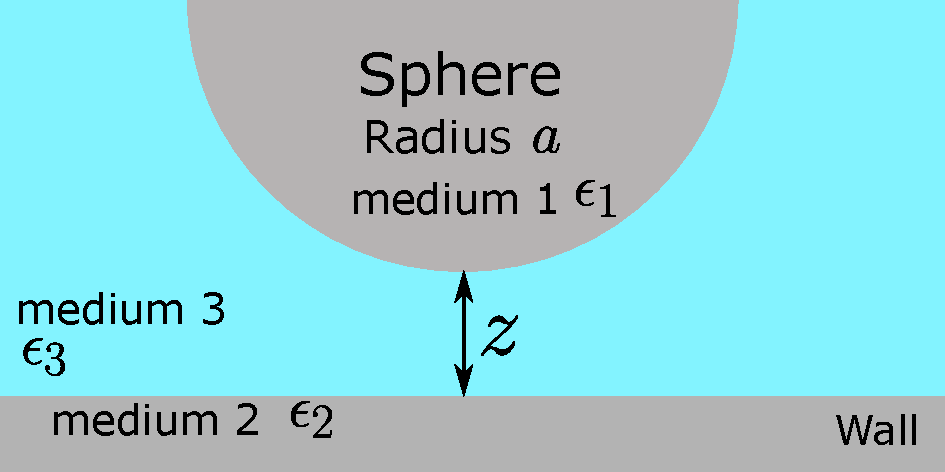
\includegraphics{02_body/chapter3/images/vdw_scheme.pdf}
	\caption{A colloid of radius $a$ is located at a distance $z$ from the wall. The dielectric constants of the sphere, wall and liquid are respectively $\epsilon_1$, $\epsilon_2$, and $\epsilon_3$. }
	\label{Fig:vdw}
\end{figure}

In the DLVO theory, van der Waals interactions, after integration over all surfaces contribute through a global Hamaker potential energy. This potential is short-ranged and attractive, in our case.The interaction potential reads: \cite{israelachvili_intermolecular_2015}:

\begin{equation}
	U_\mathrm{vdW} = -\frac{A a}{6z} 
\end{equation}

where $A$ is the nonretarded Hamaker constant. For our system, where the particle, medium and wall are different media as schematize in Fig.~\ref{Fig:vdw}, the Hamaker constant is given by \cite{israelachvili_intermolecular_2015}:

\begin{equation}
	A = \frac{3}{4} k_\mathrm{B}T \left(
	\frac{\epsilon_1 - \epsilon_3}{\epsilon_1 + \epsilon_3}
	\right)
	\left(
	\frac{\epsilon_2 - \epsilon_3}{\epsilon_2 + \epsilon_3}
	\right)
	+
	\frac{3h}{4\pi}
	\int_{\nu_1}^{\infty}
	\left(
	\frac{\epsilon_1 (j\nu) - \epsilon_3 (j\nu)}{\epsilon_1 (j\nu) + \epsilon_3 (i\nu)}
	\right)
	\left(
	\frac{\epsilon_2 (j\nu) - \epsilon_3 (j\nu)}{\epsilon_2 (j\nu) + \epsilon_3 (i\nu)}
	\right)
	\textnormal{d}\nu ~,
\end{equation}

where $\epsilon_1$, $\epsilon_2$ and $\epsilon_3$ are the static dielectric constants of the three media, $\epsilon_{1,2,3} (j\nu)$ are the  dielectric constant at a imaginary frequency $ j \nu$. The first term gives the zero-frequency energy of the Van der Waals interaction and the second term the dispersion energy. In the litterature, we found for polystyrene colloids in water near a glass substrate $A\approx k_\mathrm{B}T$. Since $A$ is positive, the interaction is attractive, moreover, we estimate that the van der Waals forces play a role only within a few nanometers from the surface ($z < 10$ nm), as commonly observed \cite{prieve_measurement_1999}. In our experiments, the Debye length $\ell _\mathrm{D}$ ($>20$ nm) is large enough for the particles to avoid this region. Therefore, in the following, the van der Waals interactions are neglected. It is possible to study the van der Waals interactions with Brownian motion, provided that one adds enough salt to have $\ell_\mathrm{D} \simeq 1$ nm. However, with such a short Debye length, all the colloids would stick to the surface and with each others, as a result of van der Waals forces. Interestingly, we have experimentally observed stuck particles. Further work on these events may lead to interesting insights about of the near-wall interactions. 



\paragraph{Total potential and equilibrium distribution}\mbox{}\\
\label{test}
\vspace{0.10cm}

If we combine the gravitational and electrostatic energy potentials the particles lie into a total energy potential $U(z)$, given by:

\begin{equation}
	U(z) = U_\mathrm{g} + U_\mathrm{elec}~.
	\label{eq:uz}
\end{equation}

By combining Eqs.~(\ref{eq:ug}),~(\ref{Eq:Uelec})~and~(\ref{eq:uz}), and adding the condition that a particle cannot go inside the wall, one finally gets:

\begin{equation}
	\frac{U(z)}{k_\mathrm{B}T} =  \left\{
	\begin{array}{l}
		\displaystyle B\,\textrm{e}^{-\frac{z}{\ell_\mathrm{D}}} + \frac{z}{\ell_\mathrm{B}}\ ,\quad \text{ for } z>0 \\
		+\infty\ ,\quad  \text{ for } z < 0
	\end{array}
	\right. \ .
	\label{Eq:PDF}
\end{equation}

From this total potential energy, one can then construct the Gibbs-Boltzmann distribution to write the equilibrium \gls{PDF} of position $P_{\mathrm{eq}}(z)$:

\begin{equation}
	P_\mathrm{eq} (z)  = A \exp \left( -\frac{U(z)}{k_\mathrm{B}T} \right) ~,
	\label{Eq.Peq}
\end{equation} 

where $A$ is a normalization constant such that $\int_{0}^{\infty}P_\mathrm{eq}(z)\textnormal{d}z = 1$. Given an ensemble of heights $z_i$, one can compute $P_\mathrm{eq}$ using the following Python function \mintinline{python}{Peq}, where the $A$ is computed using the \mintinline{python}{np.trapz} function. Examples of a theoretical energy potential and associated \gls{PDF} of position can be seen in Fig.~\ref{Fig:potential} for $\ell_\mathrm{B} = 500 ~ \mathrm{nm} $,  $B = 4$ and $\ell_\mathrm{D} = 50 ~ \mathrm{nm}$.

\begin{minted}
	[
	autogobble,
	frame=lines,
	framesep=2mm,
	baselinestretch=1.2,
	obeytabs=true,
	tabsize=2,
	fontsize=\footnotesize,
	linenos
	]
	{python}
import numpy as np
	
def _Peq(z):
	if z <= 0:
		return 0
	else:
		return np.exp(-(B * np.exp(-z / ld) + z / lb))
	
	
def Peq(z):
	P = np.array([_Peq(zi) for zi in z])
return P / np.trapz(P,z)
\end{minted}



\begin{figure}[h]
	\centering
	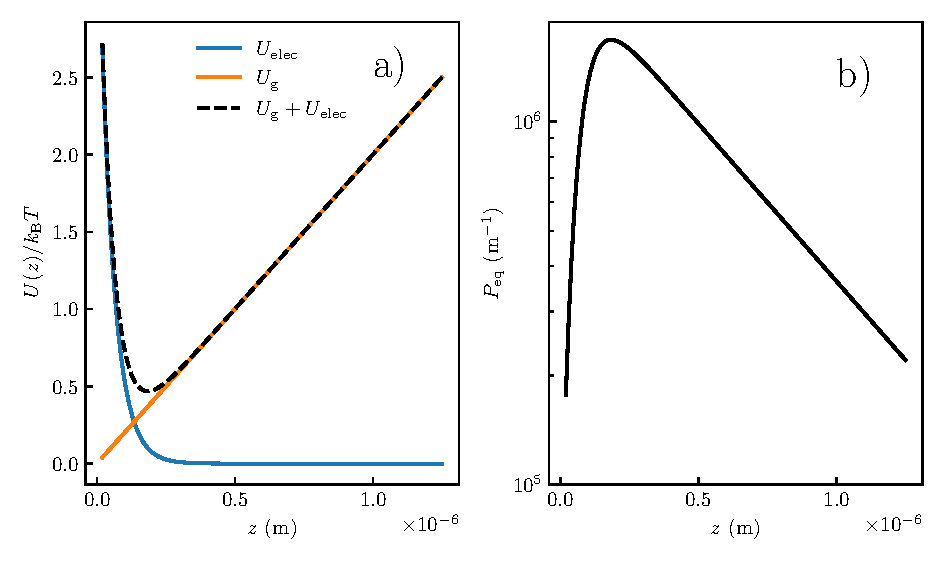
\includegraphics{02_body/chapter3/images/potential/potential_exemple.pdf}
	\caption{ a) In orange potential energy $U_\mathrm{g}$ (see Eq.~(\ref{eq:ug})) of a colloid with a Boltzmann length $\ell_\mathrm{B} = 500 ~ \mathrm{nm} $. In blue, the electrostatic potential energy $U_\mathrm{elec}$ (see Eq.~(\ref{Eq:Uelec})) is characterized by a dimensionless magnitude $B = 4$ and a Debye length $\ell_\mathrm{D} = 50 ~ \mathrm{nm}$. The dashed line corresponds to the total potential $U$, see Eq.~(\ref{eq:uz}). b) Corresponding Gibbs-Boltzmann equilibrium distribution of position calculated using the energy potential of panel a).}
	\label{Fig:potential}
\end{figure}

\newpage

\subsubsection{Local diffusion coefficient}

\begin{figure}
	\centering
	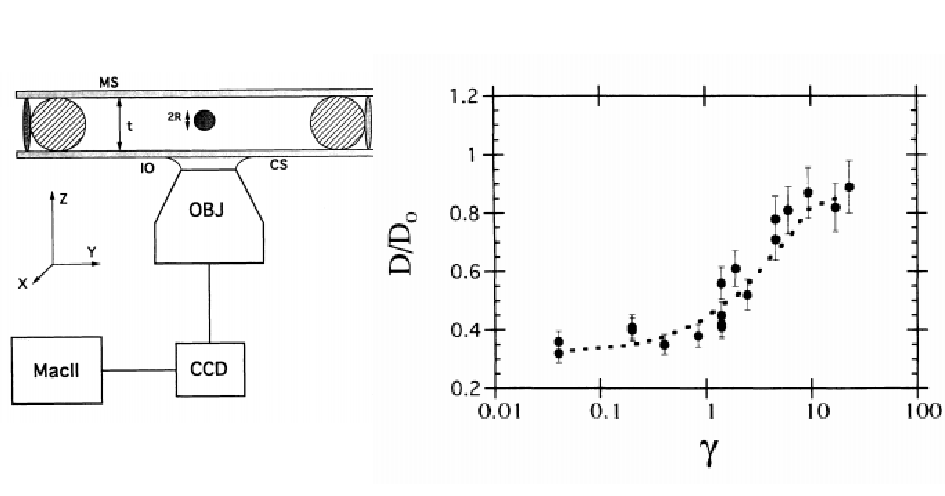
\includegraphics{02_body/chapter1/image/libchaber.pdf}
	\caption{Figure extracted from \cite{faucheux_confined_1994}. On the left is the experimental setup. It is an inverted microscope used in order to track micrometric particles of diameter $2R$ inside a liquid cell of thickness $t$. On the right is the final result, where the authors measure the diffusion parallel (\textit{i.e.} along $x$ or $y$) coefficient $D_\parallel$ (see Eqs.~(\ref{Eq:etax})~and~(\ref{Eq.hindered})), normalized by the bulk diffusion coefficient $D_0$, as a function the confinement parameter $\gamma = \langle z \rangle_t/a$, with $\langle z \rangle_t$ time-averaged particle-wall distance.}
	\label{fig:libchaber}
\end{figure}


As we have seen in Chapter~\ref{sec:chapter1}, for a freely diffusing colloid in the bulk, the diffusion coefficient is given by Eq.~(\ref{Eq:D_einstein}) and is a constant. However, when a particle is confined by a rigid wall, the diffusion is hindered. This means that the diffusion coefficient varies with the particle-wall distance and becomes anisotropic.A seminal measurement of this effect was done by Faucheux and Libchaber \cite{faucheux_confined_1994}. As we can see in Fig.~\ref{fig:libchaber}, using a microscope, they tracked colloids within a parallelepipedic chamber, and measured the thickness-averaged diffusion coefficients for different value of the confinement parameter $\gamma = \langle z\rangle_t / a$, with $\langle z \rangle_t$ time-averaged particle-wall distance. As experiments reach equilibrium, $\langle z \rangle_t$ is given by the Gibbs-Boltamann distribution as $\langle z \rangle_t = \int \textnormal{d}zP_\mathrm{eq}(z))z$. We observe that the diffusion coefficient parallel to the surface decreases as the particle gets closer to the wall, and seems to saturate around $0.3D_0$ at low $\gamma$, with $D_0$ the diffusion coefficient in the bulk (see Eq.~\ref{Eq.D}). 
\newpage

To understand the reason for this hindered diffusion coefficient, let us start by writing the diffusion coefficient $D$ using the fluctuation dissipation theorem:

\begin{equation}
	D = \mu k_\mathrm{B}T ~,
	\label{Eq.fluc}
\end{equation}

with the mobility defined as:

\begin{equation}
	\mu = \left| \frac{v_\mathrm{sphere}}{F_\mathrm{drag}} \right|~,
	\label{Eq.mu}
\end{equation}

where $v_\mathrm{sphere}$ is the terminal velocity to an applied force $F_\mathrm{drag}$. For a spherical colloid of radius $a$ moving at a velocity $v_\mathrm{sphere}$, the drag force $F_{\mathrm{drag}} ^\mathrm{B}$ is given by the Stokes' law:

\begin{equation}
	F_\mathrm{drag} ^\mathrm{B} = -c \pi \eta a v_\mathrm{sphere} ~,
	\label{Eq.drag}
\end{equation}

where $c$ is a constant that depends on the boundary conditions imposed at the surface of the colloid. Typically, one has $c = 6$ for a no-slip boundary conditions and $c = 4$ for a full-slip boundary conditions, such as for air bubbles for example. Combining Eqs.~(\ref{Eq.fluc}),~(\ref{Eq.mu})~and~(\ref{Eq.drag}) for a freely diffusing no-slip hard sphere in the bulk we retrieve Eq.~(\ref{Eq:D_einstein}): 

\begin{equation}
	D = D_0 = \frac{k_\mathrm{B}T}{6\pi \eta a} ~.
	\label{Eq.D}
\end{equation}

The Stokes' drag force can be computed by solving the Navier-Stokes equation:

\begin{equation}
	\rho \left[ \frac{\partial \vec{v}}{\partial t} + \left(\vec{v} \cdot \nabla \vec{v} \right) \right] + \nabla p = \eta \nabla ^2 \vec{v} ~,
	\label{Eq.Navier}
\end{equation}

and the continuity equation for incompressible fluids:

\begin{equation}
	\nabla \cdot \vec{v} = 0~,
	\label{Eq.continuity}
\end{equation}

where $\vec{v}$ and $p$ are receptively the velocity and pressure fields, and where $\rho$ is the liquid density. When the Reynolds number $\textnormal{Re} = \rho a v_\mathrm{sphere} / \eta \ll 1$,  the second inertial term is negligibly small compared to the viscous term $\eta \nabla ^2 \vec{v}$. In that case, and at long-enough time for the first inertial term to be negligible, the Eq.~(\ref{Eq.Navier}) is simplified to the steady Stokes equation:

\begin{equation}
	\nabla p = \eta \nabla ^2 \vec{v}~.
	\label{Eq.Stokesflow}
\end{equation}

By solving Eqs.~(\ref{Eq.continuity})~and~(\ref{Eq.Stokesflow}) with a no-slip boundary condition on the particle surface and the field vanishing at infinity, one can calculate the velocity and the pressure fields in the fluid. By integration of the pressure and viscous stress on the particle surface, one eventually gets the Stokes mobility. However, in the case of a confined particle near a wall there is an additional no-slip condition at the wall surface. At the macro scale, this effect can be seen with a frisbee, indeed, as it gets closer to the ground, hydrodynamic pressure increases due to the increasing air velocity gradient in the gap and one can observe a slowing down of the free fall.

To get some physical insight on this effect, one can use the lubrication theory to make a scaling of the drag force experience by a particle confined near a wall. As schematized in Fig.~\ref{fig.shear}, we consider a particle of radius $a$ moving at a velocity $V$. 

\begin{figure}[ht]
	\centering
	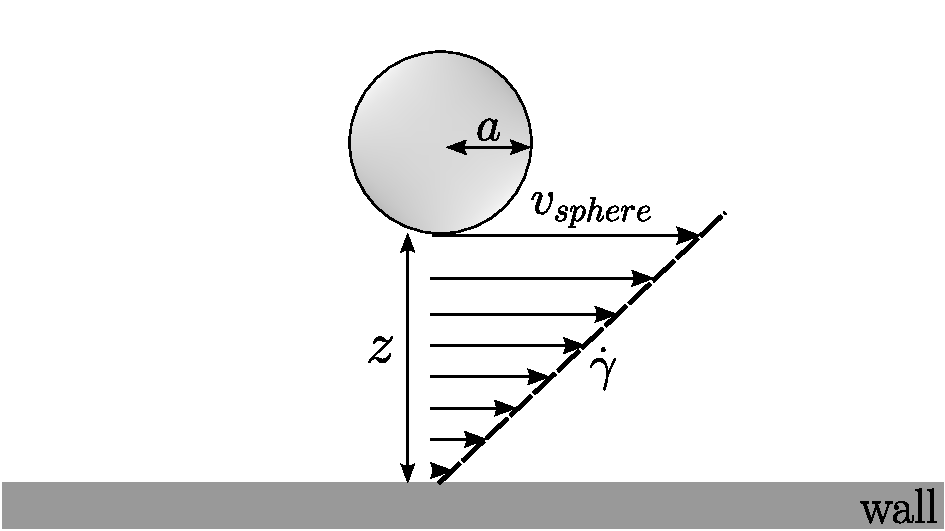
\includegraphics{02_body/chapter3/images/draw_shear/shear.pdf}
	\caption{Schematic representation of a spherical object of radius $a$ moving near a wall at velocity $V$ and inducing a fluid velocity $v_x$ and $v_z$, along the $x$- and $z$-axis, respectively.} 
	\label{fig.shear}
\end{figure}

As we are using the lubrication theory, we suppose that the particle is close to the wall such that $z \ll a$. In that condition, one has the fluid velocity along the $x$-axis $v_x \approx V$, and along the $z$-axis, $v_z \approx Vz/L \ll v_x$. Moreover, the typical length scale along the $z$-axis is the particle-wall distance $z$; and the distance $L=\sqrt{az}$ (\textit{i.e.} Hertz contact), along the $x$-axis. In this approximation, the $v_z$ terms will be negligible in Eq.~(\ref{Eq.Stokesflow}), a projection along the $z$-axis thus gives:

\begin{equation}
	\frac{\partial p}{\partial z} = 0 ~.
\end{equation}

On the right-hand side of Eq.~\ref{Eq.Stokesflow}, the viscous term simplifies to $\eta \partial_z^2 v_x $ as:

\begin{equation}
	\frac{\partial^2 v_x}{\partial x^2} \approx \frac{V}{L} \ll \frac{V}{e} \approx \frac{\partial^2 v_x}{\partial z^2}~.
\end{equation}

In the lubrication theory, Eq.~(\ref{Eq.Stokesflow}) is finally simplified to:

\begin{equation}
	\frac{\partial p}{\partial x} = \eta \frac{\partial ^2 V}{\partial z^2}~.
\end{equation}

By replacing the partial derivative by the typical length leads to:

\begin{equation}
	p \sim \eta V \frac{L}{z^2}
\end{equation}

Integrating this pressure over the particle surface (\textit{i.e} over the typical length $L = \sqrt{az}$) leads a scaling of the drag force:

\begin{equation}
	F_\mathrm{drag} ^{z\ll a} \sim \eta V \frac{L^2}{z^2} = \eta V \frac{a}{z}
\end{equation}

The mobility (see Eq.~(\ref{Eq.mu})) thus scale as $z/a$. Therefore, the diffusion coefficient of a confined colloid near a wall in the lubrication approximation is hindered and inversely proportional to the particle-wall distance.

To recap, a colloid diffusing near a wall thus experience a local drag force that depends on both its distance $z$ to the wall and direction of motion. Thanks to the linearity of the Stokes equation, one can decompose this local drag force in two contributions, for motions parallel and perpendicular to the wall. As the presence of the wall modifies the drag force with a space-dependent multiplicative factor, the confinement effect is often expressed in terms of effective viscosities:

\begin{equation}
	\eta _\bot (z) = {\eta}{\lambda _ \bot (z)}  ~ \text{, and } ~\eta _\parallel (z) =  {\eta}{\lambda _ \parallel (z)}~,
\end{equation}

where $\lambda _\bot$ and $\lambda _\parallel$ are respectively the perpendicular and parallel correction factors. Taking into account these corrections, the diffusion coefficients for perpendicular and parallel motions relative to the wall read:

\begin{equation}
	D_\bot (z) =  \frac{D_0}{\lambda _\bot (z)}  ~, \text{ and } D_\parallel (z) = \frac{D_0}{ \lambda_\parallel (z)} ~.
	\label{Eq.hindered}
\end{equation}

For no-slip boundary conditions imposed at both the wall and the surface of the colloid, Brenner \cite{brenner_slow_1961} obtained for the perpendicular motion:


\begin{equation}
	\lambda_ \bot (z) = \frac{4}{3}  \mathrm{sinh}\beta \sum _{n=1} ^{\infty} \frac{n(n+1)}{(2n-1)(2n+3)}
	\left[
	\frac
	{
		2\mathrm{sinh}(2n + 1)\beta + (2n +1)\mathrm{sinh}2\beta
	}
	{
		4\mathrm{sinh}^2(n + 1 /2)\beta  - (2n+1)^2 \mathrm{sinh}^2 \beta
	}
	-1
	\right] ~,
	\label{Eq:etaz}
\end{equation}

where $\beta = \cosh ^{-1} ((z+a)/a)$. For the motion of a sphere parallel to a wall, Faxén found \cite{faxen_fredholm_1924}:

\begin{equation}
	\lambda_\parallel(z) = 
	\left[
	1 - \frac{9}{16} \xi + \frac{1}{8}\xi^3 - \frac{45}{256}\xi^4 - \frac{1}{16}\xi^5
	\right]^{-1}~,
	\label{Eq:etax}
\end{equation}

where $\xi  = a / (z+a)$. Eqs.~(\ref{Eq:etaz})~and~(\ref{Eq:etax}) are exact for all $z$ and shown in Fig.~\ref{fig.etaz}-a). However, the solution for the perpendicular motion can be complex to compute as it is an infinite series. It requires a software that enables arbitrary-precision floating-point arithmetic\footnote{Arbitrary-precision floating-point arithmetic enables to evaluate mathematical expressions with any precision, \textit{i.e.} any number of digits.} --- such as Mathematica or the \mintinline{python}{mpmath} Python's module, for example. $D_\bot$ can be evaluated using the following Python snippet, where the \mintinline{python}|nsum| function is used to compute the summation:  


\begin{minted}
	[
	frame=lines,
	framesep=2mm,
	baselinestretch=1.2,
	fontsize=\footnotesize,
	linenos
	]
	{python}
from mpmath import nsum 
	
def Dz(eta, z, a):
  a = (z + a) / a
  beta = float(acosh(a))
  summ = nsum(
    lambda n: (n * (n + 1) / ((2 * n - 1) * (2 * n + 3)))
    * (
        (
          (2 * sinh((2 * n + 1) * xi) + (2 * n + 1) * sinh(2 * beta))
          / (
              4 * (sinh((n + 1 / 2) * beta) ** 2)
              - ((2 * n + 1) ** 2) * (sinh(beta) ** 2)
          )
    )
    - 1
  ),
  [0, inf],
  )
  summ = float(summ)
  return kT / (6 * pi * eta * 4 / 3 * float(sinh(beta)) * summ * a)

\end{minted}

To simplify the computation of $\lambda_\bot$, Goldman \textit{et al.} \cite{goldman_slow_1967} showed that Eq.~(\ref{Eq:etaz}) can be Padé approximated, giving:

\begin{equation}
	\lambda_\bot =  \frac{6z^2 + 9az + 2a^2}{6z^2 + 2az}~.
	\label{Eq:etaz_pade}
\end{equation}

In the near-wall regime, such that $z \ll a$, it is possible to further approximate $\lambda_\bot$ by its asymptotic expression:

\begin{equation}
	\lambda_\bot \simeq \frac{a}{z} ~.
	\label{Eq:etaz_small}
\end{equation}


\begin{figure}[H]
	\centering
	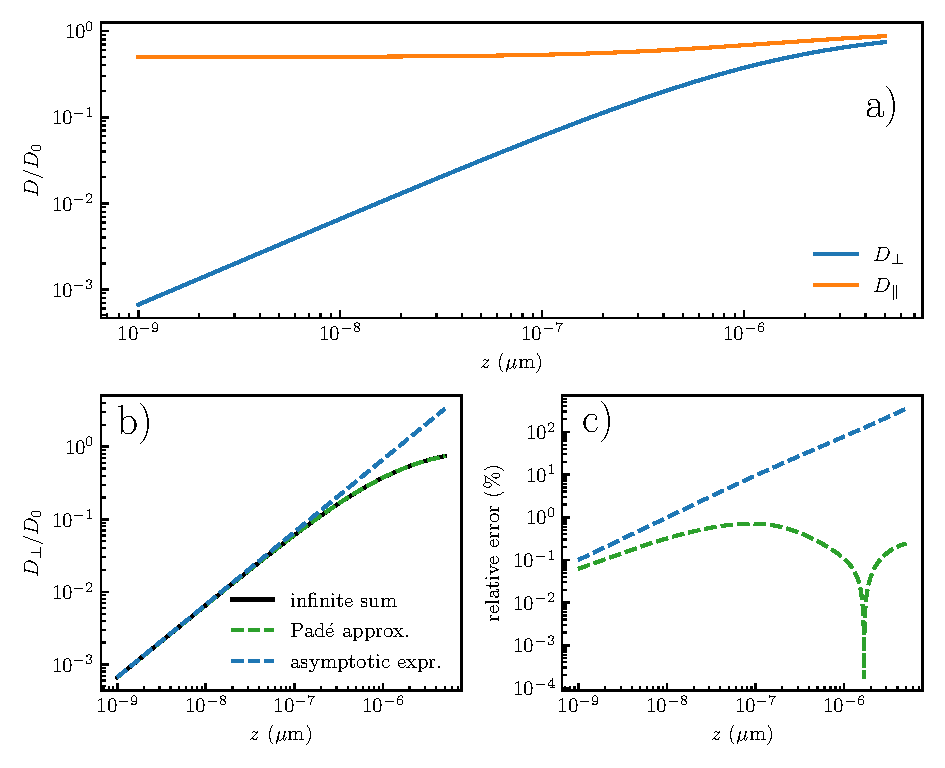
\includegraphics{02_body/chapter3/images/theory_lambda/hindered_diffusion.pdf}
	\caption{a)  Parallel and perpendicular normalized diffusion coefficients for a colloidal particle of radius $a = 1.5 ~ \mathrm{\mu m}$. b) Perpendicular normalized diffusion coefficient at a distance $z$ from a wall. The solid black line is the exact solution given by the infinite sum of Eq.~(\ref{Eq:etaz}). The green dashed line is the Padé approximation od Eq.~(\ref{Eq:etaz_pade}). The blue dahed line is the near-wall asymptotic expression of Eq.~(\ref{Eq:etaz_small}). c) Relative errors between the two approximations (dashed lines of panel b), same color code) and the exact result (solid line of panel b)).}
	\label{fig.etaz}
\end{figure}


The exact result, together with the Padé approximation and the near-wall asymptotic expression for the hindered vertical diffusion are plotted in Fig.~\ref{fig.etaz}-b). The Padé approximation fits well the exact solution, the near-wall asymptotic expression fits well when $z < a / 10$ typically. To check how precise both approximations are, we plot the relative error in Fig.~\ref{fig.etaz}-c). The Padé approximation shows precision up to 1\%. Thus, in the following, when evaluating perpendicular diffusion coefficients, or equivalently vertical effective viscosities, the Padé approximation will be used. 


\subsubsection{Langevin equation for confined Brownian motion}

Now that the external forces acting on the particle and hindered diffusion coefficients are known, we rewrite the overdamped Langevin (see Eq.~(\ref{Eq.overdamped_SDE})) as:

\begin{equation}
	V_t^i \textnormal{d}t  = -\mu(z)\frac{\partial U(z)}{\partial x_i}  \textnormal{d}t + \sqrt{2D_i (z)}  \textnormal{d}B_t ~,
	\label{Eq:langevin_z}
\end{equation}

where $\mu(z) = 1/ (6 \pi \eta_i(z) a)$, and $i$ denotes one of the three spatial directions, $x,~ y$ and $z$, where the previously determined $\eta_\parallel$ or $D_\parallel$ correspond to the $x$- and $y$-axes and $\eta_\bot$ or $D_\bot$ corresponds to the $z$-axis., and  $ \textnormal{d}B_t$ is a Gaussian-distributed satisfying $\langle \textnormal{d}B_t \rangle = 0$ and $\langle \textnormal{d}B_t ^2 \rangle = \textnormal{d}t$. As we have discussed previously, the potential $U$ only varies along the $z$-axis, thus, the external forces only acts on the particle on the $z$-axis while the particle diffuses freely along the $x$- and $y$-axis. 

\subsubsection{Spurious drift}

It is interesting to observe that due to the hindered diffusion the magnitude of the Langevin force, $\sqrt{2D_i(z)}$, is not anymore constant, but varies with the height of the particle. This effect is called multiplicative noise and will have some interesting effects on the dynamic properties of the Brownian motion. To show the effects of the multiplicative noise, one can integrate over a time $\tau$ the Eq.~(\ref{Eq:langevin_z}), in the absence of the external force one as:

\begin{equation}
	\Delta x_i = \int_{t_0} ^{t_0 + \tau} \sqrt{2D_i(z)}\textnormal{d}B_t
	\label{int}
\end{equation}

where $\Delta x_i$ is a space increment. However, the noise term is not well defined and the time at which the magnitude of the force $\sqrt{2D_i(z)}$ in the integration Eq.~(\ref{int}) needs to be specified. It is thus necessary to determine where the diffusion coefficient $D(z)$ in Eq.~(\ref{int}) is evaluated in the time interval $[t_0, t_0 + \tau]$. In general, $D(z)$ is represented by $D(z + \alpha \Delta z)$, or in the same way $D(z(t_0 + \alpha \tau))$, with $\alpha \in [0,1]$. The value of $\alpha$ determines at which time in the interval   $[t_0, t_0 + \tau]$ the local diffusion is evaluated, hence, the magnitude of the random force. The physics will thus change on how the noise is calculated; however, the requirement is that the long-time thermal equilibrium must be consistent with the Boltzmann distribution and, hence, constrain the choice of $\alpha$. Taking into account $\alpha$, removing the external forces, the Langevin equation along the $z$-axis becomes:

\begin{equation}
	\Delta z  = \sqrt{2D_\bot (z + \alpha \Delta z)} d B_t ~.
	\label{int2}
\end{equation}

By Taylor expanding $D_ \bot$ to the first order, one has:

\begin{equation}
	D_\bot (z + \alpha \Delta z) \simeq D_\bot (z)  + \alpha \frac{\textnormal{d} D_\bot(z)}{\textnormal{d}z} \Delta z ~.
\end{equation}

Substituting the later in Eq.~(\ref{int2}) leads to:

\begin{equation}
	\begin{aligned}
		\Delta z &\simeq \sqrt{2D_\bot (z)  + \alpha \frac{\textnormal{d} D_\bot(z)}{\textnormal{d}z} \Delta z} d B_t  \\
		& = \sqrt{2D_\bot (z)} \left[1 + \alpha \frac{\textnormal{d} D_\bot(z)}{\textnormal{d}z} \frac{\Delta z }{D_\bot(z)}\right] ^{-1/2} \textnormal{d} B_t  ~.
	\end{aligned}
	\label{int3}
\end{equation}

Additionally, since the last term satisfies:

\begin{equation}
	\alpha \frac{\textnormal{d} D_\bot(z)}{\textnormal{d}z} \frac{\Delta z }{D_\bot(z)} \ll 1 ~,
\end{equation}

one can thus Taylor expend at the first order the last term of Eq.~(\ref{int3}) as:

\begin{equation}
	\left[1 + \alpha \frac{\textnormal{d} D_\bot(z)}{\textnormal{d}z} \frac{\Delta z }{D_\bot(z)}\right] ^{-1/2} \simeq 1 + \frac{\alpha }{2}\frac{\textnormal{d} D_\bot(z)}{\textnormal{d}z} \frac{\Delta z }{D_\bot(z)} ~.
\end{equation}

By finally substituting the first-order expansion of $\Delta z \simeq \sqrt{2D(z)} \textnormal{d}B_t$, we obtain:

\begin{equation}
	\begin{aligned}
		\Delta z & \simeq \sqrt{2D_\bot (z)} \left[1 + \frac{\alpha }{2} \frac{\textnormal{d} D_\bot(z)}{\textnormal{d}z} \frac{\Delta z }{D_\bot(z)}\right]  \textnormal{d} B_t \\
		& \simeq \sqrt{2D_\bot (z)} \left[1 + \frac{\alpha }{2} \frac{\textnormal{d} D_\bot(z)}{\textnormal{d}z} \frac{\sqrt{2D(z)} \textnormal{d}B_t }{D_\bot(z)}\right]  \textnormal{d} B_t \\
		& =  \sqrt{2D_\bot (z)} \textnormal{d}B_t + \alpha  \frac{\textnormal{d} D_\bot(z)}{\textnormal{d}z} \textnormal{d} B_t ^2
	\end{aligned}
\end{equation}



Since for a short time $\textnormal{d}B_t \rightarrow 0$ it is possible to replace $\textnormal{d}B_t ^2$ by its average value  $\langle \textnormal{d}B_t ^2 \rangle _t = \tau$, the latter thus become \cite{ikeda_stochastic_2014}: 

\begin{equation}
	\begin{aligned}
		\Delta z &=   \alpha  \frac{\textnormal{d} D_\bot(z)}{\textnormal{d}z}  \tau - \frac{1}{\gamma(z)}\frac{\partial U(z)}{\partial z}  \tau + \sqrt{2D_\bot (z)} \textnormal{d}B_t \\
		&=  \left( - \frac{1}{\gamma(z)}\frac{\partial U(z)}{\partial z} +  \alpha  \frac{\textnormal{d} D_\bot(z)}{\textnormal{d}z} \right) \tau + \sqrt{2D_\bot (z)} \textnormal{d}B_t \\
		&= \bar{v}_\textnormal{d}\tau  + \sqrt{2D_\bot (z)} \textnormal{d}B_t ~,
	\end{aligned}
\end{equation}

where:

\begin{equation}
	\bar{v}_\textnormal{d} = - \frac{1}{\gamma(z)}\frac{\partial U(z)}{\partial z} +  \alpha  \frac{\textnormal{d} D_\bot(z)}{\textnormal{d}z}  = v_\textnormal{d} + v_\textnormal{noise}~,
	\label{Eq.total_drifts}
\end{equation}

are the total drifts acting on the particle. The first term $v_\textnormal{d}$ is the drift  due to ``real" deterministic forces due to the electrostatic double-layer and gravity interactions, while the second term $ v_\textnormal{noise}$ represents a noise-induced drift. This spurious drift does disappear when the diffusion coefficient is homogeneous, as for the $x$- and $y$-axis since the diffusion coefficient only depends on the colloid's height. Theoretically, $\alpha$ can take any value between 0 and 1. However, $\alpha$ generally takes 3 different values \cite{volpe_effective_2016}:  $\alpha = 0$, the Itô integral, corresponding to the use of the initial value of $D(z)$; $\alpha = 1/2$, the Stratonovich integral, corresponding to the mid-point value; and $\alpha = 1$ the anti-Itô or isothermal integral, corresponding to the use of the final value. 

In particular, the Itô integral $\alpha = 0$ is commonly used in economics and biology as integrals are approximated by a sum, the first point of the integral is chosen.  The Stratonovich integral $\alpha = 1/2$ arises in physical systems where noise correlation time $\tau _\mathrm{c} > 0$, and where the velocities are often computed at mid-points using three measurements. Finally, the isothermal integral $\alpha = 1$ is used in physical systems at equilibrium with a heat bath \cite{volpe_influence_2010} such as our case with Brownian motion. Using the Padé approximation Eq.~(\ref{Eq:etaz_pade}), the spurious drift $v_\textnormal{noise}$ writes:

\begin{equation}
	v_\textnormal{noise} (z)= 2 \alpha D_0 a\frac{2a^2 + 12 az + 21 z^2}{(2 a^2 + 9az + z^2) ^2} ~,
	\label{Eq.spurious_drift}
\end{equation}

and the deterministic part of the drift writes:

\begin{equation}
	v_\textnormal{d} =- \frac{k_\mathrm{B}T}{\gamma(z)} \left[- \frac{1}{\ell_\mathrm{D}} B \exp \left(- \frac{z}{\ell_\mathrm{D}}\right) + \frac{1}{\ell_\mathrm{B}}\right] ~.
\end{equation}
Finally, the Langevin equation for a confined colloid near a wall writes:

\begin{equation}
	V_t^i \textnormal{d}t  = \bar{v}_\mathrm{d} ^i \textnormal{d}t + \sqrt{2D_i (z)}  \textnormal{d}B_t ~,
	\label{Eq.langevin_confined}
\end{equation}

where the drifts $\bar{v}_\mathrm{d} ^i $ are non-zero only for the $z$-axis. A typical example of drift velocity for a colloidal particle of radius $a = 1.5 ~\mathrm{\mu m}$ in water, confined in interaction potential with a Debye length $\ell_\mathrm{D} = 50 ~ \mathrm{nm}$, $B = 4 ~k_\mathrm{B}T$ and a Boltzmann length $\ell_\mathrm{B} = 500 ~ \mathrm{nm}$, is plotted in Fig.~\ref{fig.spurious}. As one can observe, the spurious drift is not negligible.
\begin{figure}[ht]
	\centering
	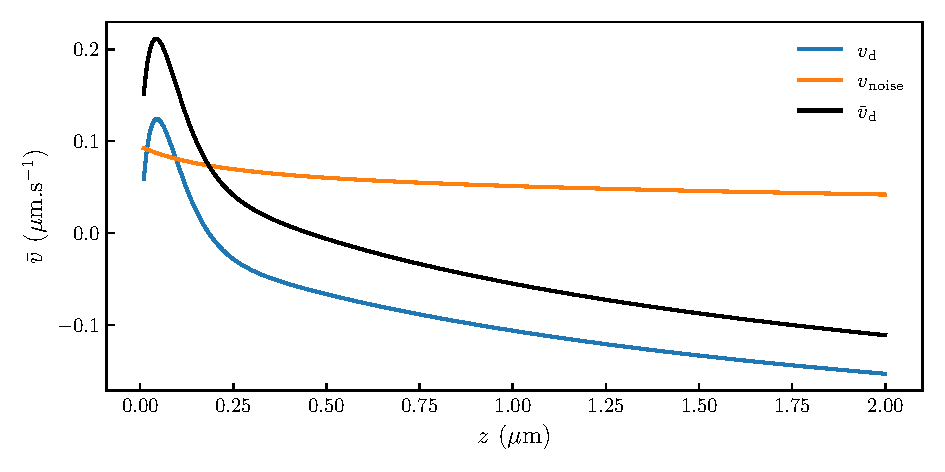
\includegraphics{02_body/chapter3/images/spurious_drift/spurious.pdf}
	\caption{Typical drift velocity for a confined colloidal particle of radius $a = 1.5 ~\mathrm{\mu m}$ in water. The physical properties of the interaction are $\ell_\mathrm{D} = 50 ~ \mathrm{nm}$, $B = 4 ~k_\mathrm{B}T$ and $\ell_\mathrm{B} = 500 ~ \mathrm{nm}$.} 
	\label{fig.spurious}
\end{figure}

\subsubsection{Fokker-Plank equation}

The Fokker-Plank equation is an alternative way to describe Brownian motion. Instead of explicitly calculating a Brownian trajectory by solving the Langevin equation, Fokker-Plank equation describes the particle distribution function $P(x, x_0; t)$ where $x$ denotes the particle position and $x_0$ its initial position. To derive the Fokker-Plank equation, let us start by taking generic Langevin equation:

\begin{equation}
	\textnormal{d}X_t = u(X_t) \textnormal{d}t + a(X_t)\textnormal{d}B_t ~,
	\label{SDE2}
\end{equation}

where $X_t$ is the particle position,  $u$ is the drift due to external forces and $a$ the magnitude of the random force. Let consider the average value of an arbitrary function $f(X_t)$ for a stochastic process obeying Eq.~(\ref{SDE2}), which started at position $x_0$ at time $t=0$, by definition \cite{le_bellac_equilibrium_2004}:

\begin{equation}
	\langle f(X_t) \rangle = \int \textnormal{d}x ~ p(x, x_0 ; t) f(x) ~,
	\label{fokker1}
\end{equation}

with the initial conditions that can be written as:

\begin{equation}
	p(x, x_0; 0) = \delta (x - x_0) ~.
\end{equation}

We now take the time derivative of Eq.~(\ref{fokker1}), starting by expending $ f$ at the $\textnormal{d}t$ as:

\begin{equation}
	\begin{aligned}
		\left\langle \frac{\textnormal{d}f(X_t)}{\textnormal{d}t} \right\rangle  &\simeq \frac{\textnormal{d}}{\textnormal{dt}}\left\langle   \frac{\partial f(X_t)}{\partial x} u(X_t) \textnormal{d}t + \frac{1}{2} \frac{\partial^2 f(X_t)}{\partial x^2} a^2 (X_t) \textnormal{d}B_t^2   \right\rangle \\
		& =  \frac{\textnormal{d}}{\textnormal{dt}} \left( \frac{\partial f(X_t)}{\partial x} u(X_t) \textnormal{d}t + \frac{1}{2} \frac{\partial^2 f(X_t)}{\partial x^2} a^2 (X_t) \textnormal{d}t \right) \\
		& = \frac{\partial f(X_t)}{\partial x} u(X_t) + \frac{1}{2} \frac{\partial^2 f(X_t)}{\partial x^2} a^2 (X_t) ~.
	\end{aligned}
	\label{fokker2}
\end{equation}

By combining Eqs.~(\ref{fokker1})~and~(\ref{fokker2}), we get:

\begin{equation}
	\begin{aligned}
		\left\langle \frac{\textnormal{d}f(X_t)}{\textnormal{d}t} \right\rangle &= \int \textnormal{d} x ~\frac{\partial p(x, x_0 ; t) }{\partial t} f(x) \\
		& =  \frac{\partial f(X_t)}{\partial x} u(X_t) + \frac{1}{2} \frac{\partial^2 f(X_t)}{\partial x^2} a^2 (X_t) \\
		& = \int \textnormal{d}x ~ p(x, x_0 ; t) G f(x) ~,
	\end{aligned}
\end{equation}

where G is an operator called the generator and is defined by its action on a function $f$ as:

\begin{equation}
	Gf = \frac{1}{2} a^2 (x) \frac{\partial ^2 f(x)}{\partial x^2} + u(x) \frac{\partial f(x)}{\partial x} ~.
\end{equation}

Using the definition of the adjoint of $G$, denoted by $G ^\dagger$, one has:


\begin{equation}
	\begin{aligned}
		\int \textnormal{d} x ~\frac{\partial p(x, x_0 ; t) }{\partial t} f(x) &= \int \textnormal{d}x ~ p(x, x_0 ; t) G f(x) \\
		&= \int \textnormal{d}x ~  G ^\dagger p(x, x_0 ; t) f(x) ~.
	\end{aligned}
\end{equation}

From the latter, we thus have:

\begin{equation}
	\frac{\partial p(x, x_0 ; t)}{\partial t} = G^\dagger p(x, x_0 ; t) ~,
	\label{fokker3}
\end{equation}

which leads to the Forward-Fokker-Planck equation:

\begin{equation}
	\frac{\partial p(x, x_0 ; t)}{\partial t }= \frac{\partial ^2}{\partial x^2} \left[\frac{a^2 (x)}{2}p(x, x_0 ; t)\right] - \frac{\partial}{\partial x} \left[u(x) p(x, x_0 ; t)\right] ~.
	\label{Eq.Forward_Fokker_plank}
\end{equation}

The latter is called Forward because the partial differential equation is in terms of the variable $x$, the position of the particle at which the stochastic process ends up, at time $t$. For a confined Brownian motion near a wall, using the previously determined drifts $\bar{v}_\textnormal{d}$ Eq.~(\ref{Eq.total_drifts}), the Fokker-Plank equation for the movement along the $z$-axis, perpendicular to the wall writes:

\begin{equation}
	\frac{\partial p(z, z_0 ; t)}{\partial t} = \frac{\partial ^2}{\partial z ^2} \left[ D(z)  p(z, z_0 ; t) \right]   -  \frac{\partial }{\partial z} \left[\bar{v}_\textnormal{d} p(z, z_0 ; t)\right] ~.
\end{equation}

As an example, the stationary solution of the latter, $\partial p / \partial t = 0$, is given by the Gibbs-Boltzmann distribution $P_\textnormal{eq}(z) $ (see Eq.~(\ref{Eq.Peq})). The solution for the Eq.~(\ref{fokker3}) with the particle starting at position $z_0$, at time $t_0 = 0$ writes:

\begin{equation}
	\begin{aligned}
		P(z, z_0; t) &= \exp (G^\dagger t) p(z, z_0, 0) \\
		& = \exp \left( \frac{\partial ^2}{\partial z ^2}  D(z)  t   -  \frac{\partial }{\partial z} \bar{v}_\textnormal{d} t\right) \delta (z - z_0)
	\end{aligned}
	\label{Eq.solfokker}
\end{equation} 

\subsubsection{Numerical simulations of confined Brownian motion}

We had previously determined that the simulation of a bulk Brownian motion without external forces can be simulated using Eq.~(\ref{Eq.shortnumlangevin}): 

\begin{equation}
	x_i = x_{i-1} + \sqrt{2D}w_i~.
\end{equation}

However, with the confined Brownian motion one needs to take into account the hindered diffusion, external forces due to gravity and double-layer interactions and the noise-induced drift. Putting all that together, leads to a new equation for $x_i$ which writes for the movement parallel to wall:

\begin{equation}
	x_i = x_{i-1} +  \sqrt{2D_\parallel}w_i ~,
\end{equation}

For the particle movement perpendicularly to the wall ($z$-axis), one needs to add the total drift $\bar{v}_\textnormal{d}$ Eq.~(\ref{Eq.total_drifts}), such that:

\begin{equation}
	z_i = z_{i-1} + \bar{v}_\mathrm{d}(z_{i-1}) \tau + \sqrt{2D_\bot}w_i ~,
\end{equation}

where $\tau$ is the simulation time step and $w_i$ being a Gaussian distributed number of mean value $\langle w_i \rangle = 0$ and variance $\langle w_i ^2\rangle = \tau$. Unlike the bulk Brownian motion where the time step $\tau$ can be chosen for the desired precision as shown previously on Fig.~\ref{fig:MSEwi}. For an accurate simulation, the time step should be short enough for the drifts $\bar{v}_\textnormal{d}$ and local diffusion coefficient to be relatively constant in the time period $t_{i+1} - t_i = \tau$ and in the displacement range $\Delta z = z_{i+1} - z_i$, such that:

\begin{equation}
	\bar{v}_\mathrm{d} (z \in [z_i, z_{i+1}]) \simeq \bar{v}_\mathrm{d} (z_i) ~,
	\label{driftc}
\end{equation}

and:

\begin{equation}
	D_{\bot, \parallel}(z \in [z_i, z_{i+1}]) \simeq D_{\bot, \parallel}(z_i) ~.
\end{equation}

Since that the diffusion coefficient varies less for the movement parallel, one can only consider the perpendicular motion to determine the simulation time step. Also, as it can be seen in Fig.~\ref{fig.taumax} where the drift $v_\textnormal{d}$ and diffusivity gradient are plotted, the diffusion gradient is negligible compared to the drift gradient, we thus focus on the drifts condition Eq.~(\ref{driftc}). Moreover, the drifts vary more when the colloid is near the surface where one can approximate the diffusion coefficient $D_\bot$ using Eq.~(\ref{Eq:etaz_small}) such that:

\begin{equation}
	\left.D_\bot  (z)\right|_{z\ll a} = D_ 0 \frac{z}{a} ~.
\end{equation}

Near the surface, the gravitational interaction can be neglected as it is smaller than the electrostatic interactions as shown in Fig.~\ref{Fig:potential}. In that case, by taking $\alpha = 1$, the total drifts Eq.~(\ref{Eq.total_drifts}) near the surface simplifies to:

\begin{equation}
	\begin{aligned}
		\bar{v}_\textnormal{d} &=  \frac{k_\mathrm{B}T}{\gamma_0} \frac{z}{a} \left[\frac{B}{\ell_\mathrm{D}} \exp \left(-\frac{z}{\ell_\mathrm{D}}\right)\right] + \frac{\partial}{\partial z} D_0 \frac{z}{a} \\
		&= D_0 \frac{z}{a} \left[\frac{B}{\ell_\mathrm{D}} \exp \left(-\frac{z}{\ell_\mathrm{D}}\right)\right] + \frac{D_0}{a} \\
		&= \frac{D_0}{a} \left[ 1 + \frac{Bz}{\ell_\mathrm{D}} \exp \left(-\frac{z}{\ell_\mathrm{D}}\right)\right]
	\end{aligned}
\end{equation}

By expending the exponential term to the order $z/\ell_\mathrm{D}$ order, we get:

\begin{equation}
	\begin{aligned}
		\bar{v}_\textnormal{d} &= \frac{D_0}{a} \left[ 1 + \frac{Bz}{\ell_\mathrm{D}} \exp \left(-\frac{z}{\ell_\mathrm{D}}\right)\right]
		=  \frac{D_0}{a} \left[ 1 + \frac{Bz}{\ell_\mathrm{D}}  \left(1 -\frac{z}{\ell_\mathrm{D}}\right)\right] \\
		& = \frac{D_0}{a} \left( 1 + \frac{B z}{\ell_\mathrm{D}}\right)
	\end{aligned}
	\label{drifts_short}
\end{equation}

To satisfy Eq.~(\ref{driftc}), we need to have small relative change of drifts in an interval $[z, z+\Delta z]$ which can be written as \cite{matse_state-dependent_nodate}:

\begin{equation}
	\frac{|\bar{v}_\mathrm{d} (z + \Delta z) - \bar{v}_\mathrm{d} (z)|}{\bar{v}_\mathrm{d} (z)} \ll 1
	\label{condition_drift}
\end{equation}

Combining Eqs.~(\ref{drifts_short})~and~(\ref{condition_drift}), we get:

\begin{equation}
	|\Delta| z \ll \frac{\ell_\mathrm{D}}{B} + z ~.
	\label{inegality}
\end{equation}


Using the \gls{MSD}, it is possible to link the latter to the simulation time step $\tau$ by using the average value of $\Delta z ^2 $, such that:

\begin{equation}
	\langle \Delta z ^2 \rangle (z) = 2 D_\bot (z) \tau = 2D_0 \frac{z}{a}\tau 
	\label{msdshort}
\end{equation}

Combining Eqs.~(\ref{inegality})~and~(\ref{msdshort}) thus leads to:

\begin{equation}
	\tau = \frac{a\langle \Delta z ^2 \rangle }{2 D_0 z} < \frac{a}{2 D_0 } \frac{(\frac{\ell_\mathrm{D}}{B} + z) ^2}{z} = \tau_\mathrm{max} (z)~,
	\label{taumax}
\end{equation}

where $ \tau_\mathrm{max}$ is thus the maximal time step that satisfies Eq.~(\ref{inegality}). At this point, there are two different ways to do the simulation: the first one is to do an adaptive time step where $\tau_\mathrm{max}$ for each step of the simulation ; the second one is to find the smallest $\tau_\mathrm{max}(z)$ and use for all the simulation a time step $\tau$ satisfying $\tau < \mathrm{min}(\tau_\mathrm{max}) $. The latter can be evaluated by finding the height $z_\mathrm{min}$, at which the derivative of $ \tau_\mathrm{max}$ nullifies, such that:

\begin{equation}
	\left. \frac{\partial \tau_\mathrm{max}}{\partial z} \right| _{z_\mathrm{min} }= 0 ~.
\end{equation} 

Solving the latter gives:

\begin{equation}
	z_\mathrm{min} = \frac{\ell_\mathrm{D}}{B} ~.
\end{equation}


which finally gives a maximal simulation time step, $\mathrm{min}(\tau_\mathrm{max})$:

\begin{equation}
	\mathrm{min}(\tau_\mathrm{max}) =  \frac{2 a}{D_0} \frac{\ell_\mathrm{D}}{B} ~,
\end{equation}

this time should be the maximal time step $\tau$ used for a confined Brownian simulation near a wall to ensure an accurate simulation of the near-wall effects. In the Fig.~\ref{fig.taumax}-b) some typical $\tau_{\mathrm{max}}$ are plotted for a colloid of radius $a=1.5 ~\mathrm{\mu m}$, $B = 4$ and $\ell _\mathrm{D}$ varying between $20$ and $100$ nm. We can observe that for this range of values that well represents the experiments that I have done during my thesis, taking a simulation time step $\tau < 0.01 ~ \mathrm{s}$ can be used for all set of parameters.


\begin{figure}[ht]
	\centering
	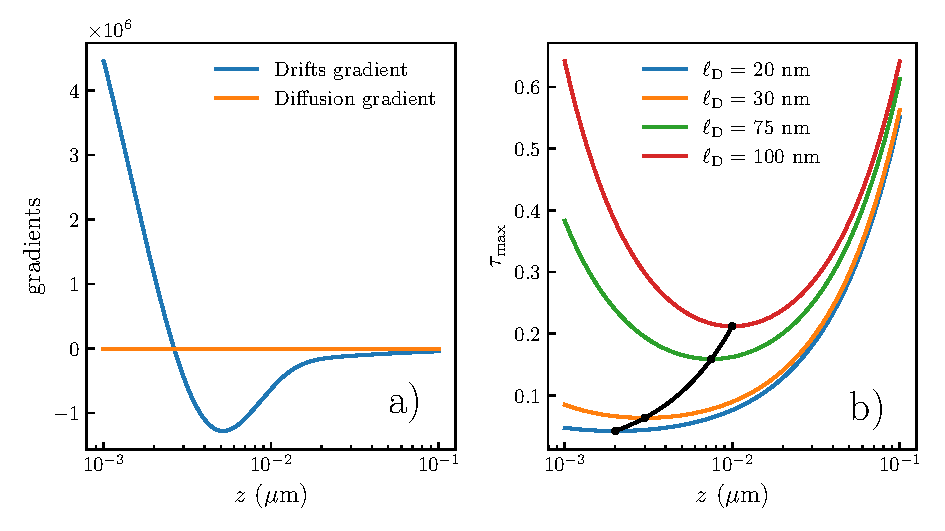
\includegraphics{02_body/chapter3/images/simulation_confined_Brownian_motion/maximal_tau.pdf}
	\caption{a) Drift and diffusive gradients for a confined colloidal particle of radius $a = 1.5 ~\mathrm{\mu m}$ in water. The physical properties of the interaction are $\ell_\mathrm{D} = 50 ~ \mathrm{nm}$, $B = 4 ~k_\mathrm{B}T$ and $\ell_\mathrm{B} = 500 ~ \mathrm{nm}$. b) $\tau_\mathrm{max}$ for a particle of radius $a = 1.5 ~\mathrm{\mu m}$ and $B = 4$ for different Debye length. The black line represents the minimum value $\tau_\mathrm{max}$ for $\ell_\mathrm{D}$ varying between 20 nm and 100 nm, this minimal time represents the maximal simulation time step that should be used for an accurate simulation.} 
	\label{fig.taumax}
\end{figure}

\begin{figure}[H]
	\centering
	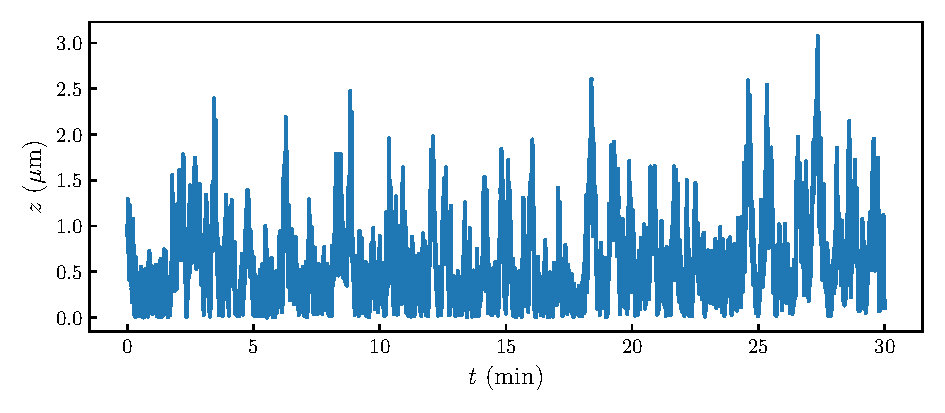
\includegraphics{02_body/chapter3/images/simulation_confined_Brownian_motion/z_traj_sim.pdf}
	\caption{Simulated confined Brownian motion height trajectory of a colloidal particle of radius $a= 1.5  ~ \mathrm{\mu m}$ of density $\rho_\mathrm{p} = 1050  ~\mathrm{kg.m^{-3}}$, $\alpha = 1$ and  the potential is characterized by $\ell_\mathrm{D} = 50$ nm and $B=4$.} 
	\label{fig.z_traj_confined_simulated}
\end{figure}

We have developed the simulation of the Confined Brownian motion using Python, as part of the Master's internship of Élodie Millan, the interested reader will find more information on confined Brownian motion in more complex systems in her forthcoming thesis. A trajectory of a colloidal particle of radius $a= 1.5  ~ \mathrm{\mu m}$ of density $\rho_\mathrm{p} = 1050  ~\mathrm{kg.m^{-3}}$ and the potential characterized by $\ell_\mathrm{D} = 50$ nm and $B=4$,  is plotted in the Fig.~\ref{fig.z_traj_confined_simulated} which does look like the experimental trajectory that was shown in Fig.~\ref{Fig:exp_z_traj} as an introduction to the chapter. In this trajectory, the noise induced lift is taken into account by using the isothermal approach $\alpha =1 $. However, to check if it is the correct way to take into account the spurious drift, the constraint we have is that the long-time statistics should satisfy the Gibbs-Boltzmann equation Eq.~(\ref{Eq.Peq}). To compute an experimental probability density function from a set of points, one can use the following Python snippet.


\begin{minted}
	[
	frame=lines,
	framesep=2mm,
	baselinestretch=1.2,
	fontsize=\footnotesize,
	linenos
	]
	{python}
	def pdf(data, bins=10, density=True):
	
	pdf, bins_edge = np.histogram(data, bins=bins, density=density)
	bins_center = (bins_edge[0:-1] + bins_edge[1:]) / 2
	
	return pdf, bins_center
\end{minted}

The Gibbs-Boltzmann distribution for $\alpha = 0 , 0.5 \text{ and } 1 $ is shown in Fig.~\ref{fig.pdf_vs_alpha}. We see that the Isothermal integral of the noise gives the correct distribution, in the other two cases, we observe that the particle is more likely to be found nearer the surface, this is corrected by the additional spurious drift Eq.~(\ref{Eq.spurious_drift}).

\begin{figure}[h!]
	\centering
	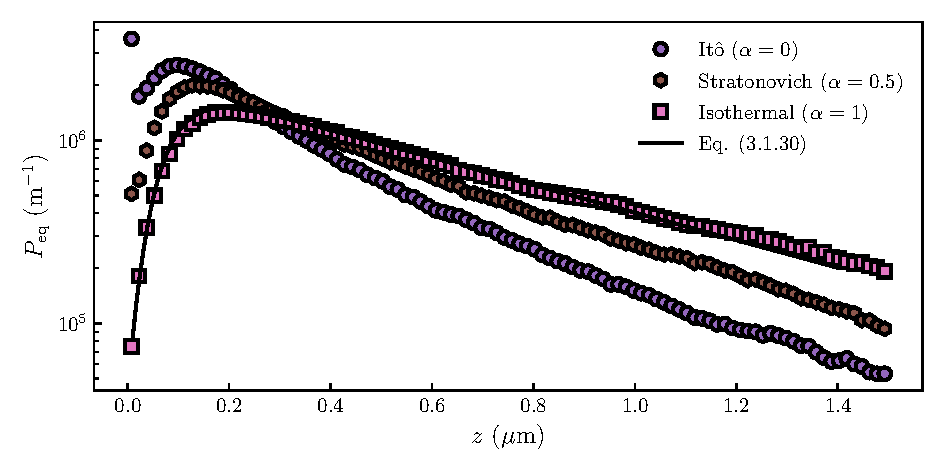
\includegraphics{02_body/chapter3/images/simulation_confined_Brownian_motion/Peq_vs_alpha.pdf}
	\caption{Probability Density Function of the height of the particle for different computation of the spurious drift, Itô $\alpha = 0$, Stratonovich $\alpha = 0.5$ and Isothermal $\alpha = 1$. The plain black line represents the expected Gibbs-Boltzmann distribution. The simulation parameters : $a = 1.5 ~ \mathrm{\mu m}$, $\rho_\mathrm{p} = 1050 ~\mathrm{kg.m^{-3}}$, $\ell_\mathrm{D} = 50$ nm, $B = 4$ and $\ell_\mathrm{B} = 577$ nm. }
	\label{fig.pdf_vs_alpha}
\end{figure}


\subsection{Experimental study}
\label{section:expresults}
Let us now analyze the experimental data obtain through the Mie tracking. In the theory, we wrote the height of the particle $z$ being the shortest distance between the wall and the colloidal particle surface. However, it is not the height measured by the Mie tracking, since it measures the distance between the objective lens focal plane and the particle center. To have the correct measured height, we suppose that the particle does approach very closely to the wall. From that assumption, we then a moving-minimum along the trajectory to set the minimal value of the trajectory to zero. The moving minimum can be calculated using the following Python function:



\begin{minted}
	[
	frame=lines,
	framesep=2mm,
	baselinestretch=1.2,
	fontsize=\footnotesize,
	obeytabs=true,
	tabsize=2,
	linenos
	]
	{python}
def movmin(z, window):
	result = np.empty_like(z)
	start_pt = 0
	end_pt = int(np.ceil(window / 2))
	
	for i in range(len(z)):
		if i < int(np.ceil(window / 2)):
			start_pt = 0
		if i > len(z) - int(np.ceil(window / 2)):
			end_pt = len(z)
			
		result[i] = np.min(z[start_pt:end_pt])
		start_pt += 1
		end_pt += 1
		return result
\end{minted}

In the latter, \mintinline{python}{window} represent the number of points is used to compute the minimum. As an example, if one chose \mintinline{python}{window = 10000}, the first value of \mintinline{python}{result} is the minimum of the first 10000 points of \mintinline{python}{z}. If there is enough data around the point where the minimum is calculated, the ensemble is centered, with a window of 100, the minimal value at the 100th elements is between the 50th and 150th (\textit{e.g.} \mintinline{python}|result[100] = np.min(z[50:150])|. The raw and rescaled trajectory are shown Fig.~\ref{fig.rescaled_traj}. Of course, that technique is not perfect and we are working on a method that could directly measure the wanted wall-particle distance, also using Mie. However, subtract the moving minimum has a benefit, indeed it can remove some experimental drift that can be due to the physical movement of the optical pieces of the microscope. Moreover, as the exact location of the $z=0$ origin is thus \textit{a priori} undetermined we add to the physical parameters $B$, $\ell_\mathrm{D}$ and $\ell_\mathrm{B}$ a height offset $z_\mathrm{off}$ that accounts for the correction of the wall position.

\begin{figure}[ht]
	\centering
	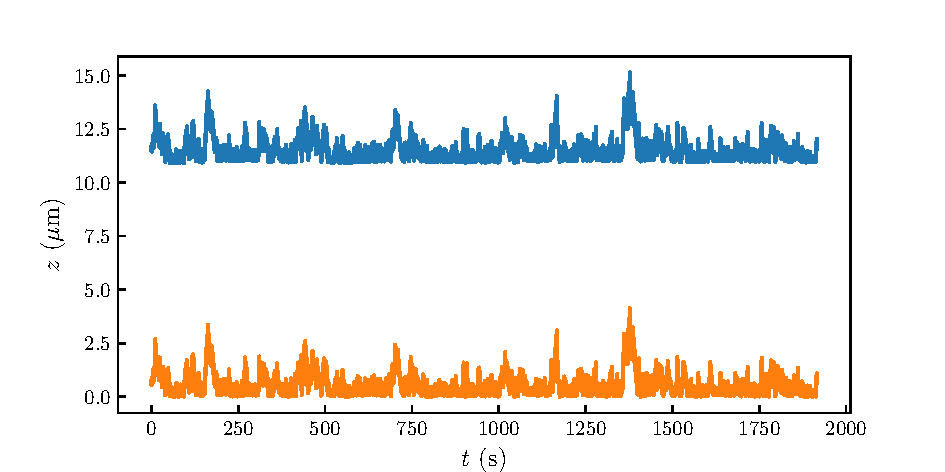
\includegraphics{02_body/chapter3/images/trajctory_analysis/traj_rescaled.pdf}
	\caption{Raw trajectory measured using the Mie tracking technique, and it's rescaled value using moving minimum algorithm with a window of $10000$ points.} 
	\label{fig.rescaled_traj}
\end{figure}

\subsubsection{Equilibrium distribution}

As we have done for the simulated trajectory, one can construct the equilibrium probability density function $P_\mathrm{eq}(z)$ of the position of the particle. As seen in Fig.~\ref{fig.pdf_exp}, and explain in the previous section, an exponential tail is observed at large distance, which is identified to the sedimentation contribution in Perrin's experiment~\cite{perrin_les_2014}, but here with the probability density function of a single particle instead of the concentration field. In contrast, near the wall, we observe an abrupt depletion, indicating a repulsive electrostatic contribution. Additionally, we see that the Gibbs-Boltzmann distribution Eq.~(\ref{Eq:PDF}) fits the data very well.



Moreover, as shown in Fig.~\ref{fig.ld}, we verified that we recover the Debye relation $\ell_{\mathrm{D}}=0.304/\sqrt{\textrm{[Nacl]}}$, with $\ell_{\mathrm{D}}$ in nm, and where [NaCl] is the concentration of salt in mol/L, with a prefactor corresponding to a single monovalent salt in water at room temperature~\cite{israelachvili_intermolecular_2015}. Besides, we have verified, as shown in Fig.~\ref{fig.ld}, that the dimensionless parameter $B$ related to surface charges is constant in the studied salt-concentration range, thus excluding any nonlinear effect~\cite{wang_measurement_2011,oberholzer_grand_1997} in our case. 

\begin{figure}[h!]
	\centering
	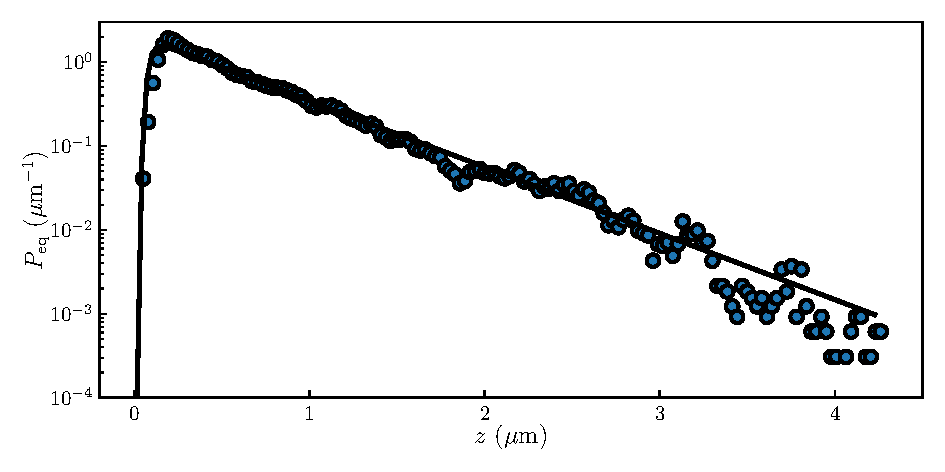
\includegraphics{02_body/chapter3/images/trajctory_analysis/pdf_exp.pdf}
	\caption{Measured equilibrium probability density function $P_{\textrm{eq}}$ of the distance $z$ between the particle and the wall. The solid line represents the best fit to the normalized Gibbs-Boltzmann distribution in position, using the total potential energy $U(z)$ of Eq.~(\ref{Eq:PDF}), with $B = 4.8$, $\ell_\mathrm{D} = 21 ~ \mathrm{nm}$, and $\ell_\mathrm{B} = 530~ \mathrm{nm}$.}
	\label{fig.pdf_exp}
\end{figure}


\begin{figure}[H]
	\centering
	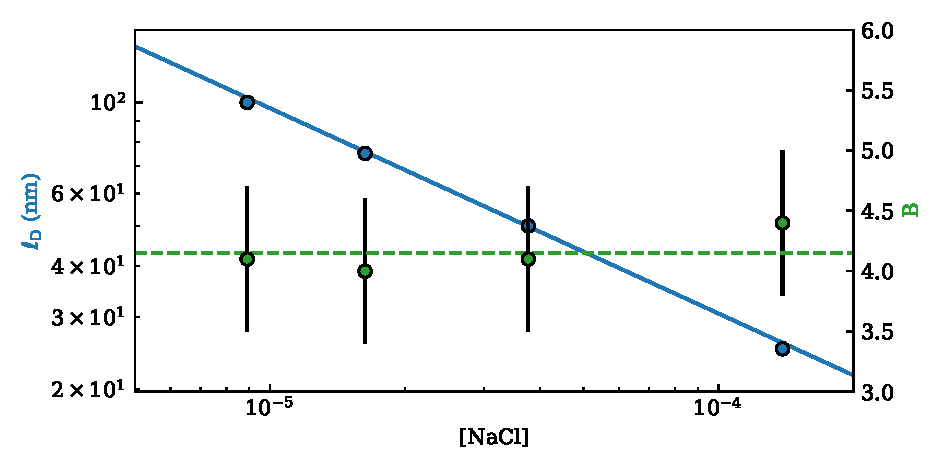
\includegraphics{02_body/chapter3/images/trajctory_analysis/ld.pdf}
	\caption{In blue, left axis, measured Debye length $\ell_\mathrm{D}$ as a function of salt concentration [NaCl]. The solid line is the expected Debye relation $\ell_\mathrm{D}=0.304/\sqrt{\textrm{[Nacl]}}$, for a single monovalent salt in water at room temperature. In green, right axis, measured $B$ as a function of salt  concentration [NaCl]. The dashed line represents the mean value of the measured $B$ values.}
	\label{fig.ld}
\end{figure}


\subsubsection{Mean Square Displacement}

We now turn to dynamic aspects, by considering the mean-squared displacement (MSD). For the three spatial directions, indexed by $i=x$, $y$, and $z$, corresponding to the coordinates $r_x=x$, $r_y=y$, and $r_z=z$, of the position $\vec{r}$, and for a given time increment $\Delta t$, the MSD is defined as:
\begin{equation}
	\langle\Delta r_i(t)^2 \rangle_t = \langle[r_i(t+\Delta t) - r_i(t)]^2\rangle_t\ ,
	\label{MSDdef}
\end{equation}
where the average $\langle\rangle_t$ is performed over time $t$. For a free Brownian motion in the bulk, and in the absence of other forces than the dissipative and random ones, the \gls{MSD} is linear in time, \textit{i.e.} $\langle\Delta r_i(t)^2 \rangle_t = 2 D_0 \Delta t$, where $D_0=k_\mathrm{B}T/(6\pi\eta a)$ is the bulk diffusion coefficient given by the Stokes-Einstein relation~\cite{einstein_uber_1905}, and $\eta$ is the liquid viscosity. Further including sedimentation restricts the validity of the previous result along $z$ to short times only, \textit{i.e.} for $\Delta t\ll\ell_{\textrm{B}}^2/D_0$ such that the vertical diffusion is not yet affected by the gravitational drift.

The presence of a rigid wall at $z=0$ adds a repulsive electrostatic force along $z$. It also decreases the mobilities nearby through hydrodynamic interactions, leading to effective viscosities $\eta_\parallel(z)=\eta_x(z)=\eta_y(z)$, and $\eta_\bot(z) = \eta_z(z)$. Interestingly, despite the previous modifications, the temporal linearity of the MSD is not altered by the presence of the wall~\cite{chubynsky_diffusing_2014,prieve_measurement_1999} for $x$ and $y$, as well as at short times for $z$. In such cases, the MSD reads:
\begin{equation}
	\langle\Delta r_i(t)^2 \rangle_t = 2 \langle D_i \rangle \Delta t\ ,
	\label{averagediff}
\end{equation}
where for each spatial direction we introduced the local diffusion coefficient $D_i(z)=D_0\eta /\eta _i(z)$, and its average 

\begin{equation}
	\langle D_i(z) \rangle = \int_0^{\infty} \textrm{d}z\, D_i(z)P_{\textrm{eq}}(z) ~,
\end{equation}  

against the Gibbs-Boltzmann distribution in position. As shown in Fig.~\ref{fig.MSD}, the MSD measured along $x$ or $y$ is indeed linear in time. By fitting the data to Eq.~(\ref{averagediff}), using Eqs.~(\ref{Eq:PDF})~and~(\ref{Eq:etax}), we extract an average transverse diffusion coefficient $\langle D_\parallel \rangle= \langle D_x\rangle=\langle D_y \rangle= 0.52\, D_0$. In contrast, along $z$, we identify two different regimes: one at short times, where the \gls{MSD} is still linear in time, with a similarly obtained best-fit value of $\langle D_z \rangle= 0.24\, D_0$; and one at long times, where the MSD saturates to a plateau. This latter behavior indicates that the equilibrium regime has been reached, with the particle having essentially explored all the relevant positions given by the Gibbs-Boltzmann distribution.

\begin{figure}[t!]
	\centering
	\includegraphics{02_body/chapter3/images/trajctory_analysis/msd.pdf}
	\caption{Measured mean-squared displacements (MSD, see Eq.~(\ref{MSDdef})) as functions of the time increment $\Delta t$, for the three spatial directions, $x$, $y$, and $z$. The solid lines are best fits to Eq.~(\ref{averagediff}), using Eqs.~(\ref{Eq:PDF}),~(\ref{Eq:etaz})~and~(\ref{Eq:etax}), with $B = 4.8$, $\ell_\mathrm{D} = 21 ~ \mathrm{nm}$, and $\ell_\mathrm{B} = 530~\mathrm{nm}$,
		providing the average diffusion coefficients $\langle{D_\parallel}\rangle= \langle D_x\rangle=\langle D_y \rangle =0.52\,D_0$ and $\langle D_z \rangle =0.24\, D_0$. The dashed line is the best fit to Eq.~(\ref{Eq:plateau}), using Eq.~(\ref{Eq:PDF}), with $B = 4.8$, $\ell_\mathrm{D} = 21 ~ \mathrm{nm}$, and $\ell_\mathrm{B} = 530~\mathrm{nm}$.}
	\label{fig.MSD}
\end{figure}


\subsubsection{Non-Gaussian dynamics - Displacement distribution}

Having focused on the \gls{MSD}, \textit{i.e.} on the second moment only, we now turn to the full probability density function $P_i$ of the displacement $\Delta r_i$. Since the diffusion coefficient $D_i(z)$ varies as a result of the variation of $z$ along the particle trajectory, $P_i$ exhibits a non-Gaussian behavior, as seen in Figs.~\ref{fig.displacement}-a,b,c,d). We even resolve the onset of a non-Gaussian behavior in $P_x$, by zooming on the large-$\lvert\Delta x\rvert$ wings. At short times, the diffusion coefficient $D_i$ and the drift velocity $\bar{v}_\mathrm{d}$, can be considered constant. By writing the initial condition $\delta(x_i - x_i ^0)$, the solution of the Forward Fokker-Plank Eq.~(\ref{Eq.solfokker}), becomes:

\begin{equation}
	\begin{aligned}
		P(x_i, z_0, \Delta t) &= \exp \left[  \frac{\partial ^2}{\partial z ^2} D_i(z_0) \Delta t - \frac{\partial}{\partial z} \bar{v}^i _\mathrm{d} (z_0) \Delta t \right] \frac{1}{2 \pi} \int _{-\infty} ^{\infty} ~ \textnormal{d}u \exp (ju(z-z_0))  \\
		&= \frac{1}{2\pi} \int _{-\infty} ^{\infty} ~ \textnormal{d}u  \left[ D_i(z_0) \Delta t \frac{\partial ^2}{\partial z ^2} \exp (ju(z-z_0)) -  \bar{v}^i _\mathrm{d} (z_0) \Delta t \frac{\partial}{\partial z} \exp (ju(z-z_0)) \right] \\
		& = \frac{1}{2\pi} \int_{-\infty}^{\infty} ~ \textnormal{d}u \exp \left[ -u^2 D(z_0)\Delta t + ju(z-z_0) - ju  \bar{v}^i _\mathrm{d} (z_0) \Delta t \right] ~,
	\end{aligned}
\end{equation}

where $ \bar{v}^i _\mathrm{d} (z_0)$ is non-zero only for the $z$-axis. The latter can be reduced to \cite{matse_state-dependent_nodate, risken_fokker-planck_2012}:

\begin{equation}
	P_i(\Delta r_i, z_0, \Delta t) =   \frac{1}{\sqrt{4 \pi D_i(z_0) \Delta t}} \exp \left[-\frac{(\Delta r_i - \bar{v}^i_\mathrm{d}\Delta t)^2}{4 D_i(z) \Delta t}   \right]\ .
	\label{Pdxshort}
\end{equation}

Which is a Gaussian distribution with a 0 mean value for the $x$- and $y$-axis and  
\begin{equation}
	\langle P_z(\Delta z, z_0, \Delta t) \rangle = \bar{v}_\mathrm{d} \Delta t ~,
\end{equation}
for the $z$-axis. Additionally, it has a variance $\sigma_i(z_0) = \sqrt{2D_i (z_0) \Delta t}$. From Eq.~(\ref{Pdxshort}), we can observe than the total drift $\bar{v}_\mathrm{d}$ induces an asymmetry on the displacement along the $z$-axis. However, in our experiment, as we have access to long enough trajectory, we are interested in the distribution which is not conditioned by the initial position but by the Gibbs-Boltzmann distribution Eq.~(\ref{Eq:PDF}). At short times, $P_i$ can thus be modeled by the averaged diffusion Green's function~\cite{matse_test_2017,hapca_anomalous_2009}:
\begin{equation}
	\begin{aligned}
		P_i(\Delta r_i, \Delta t) & = \int _{0} ^\infty ~\textnormal{d} z_0 P_\mathrm{eq}  P(x_i, z_0, \Delta t) \\
		&= \int ^\infty _0 \mathrm{d}z\, P_{\textrm{eq}}(z) \frac{1}{\sqrt{4 \pi D_i(z) \Delta t}} \textrm{e}^{-\frac{\Delta r_i^2}{4 D_i(z) \Delta t}     }\ ,
	\end{aligned}
	\label{Eq:PDzshort}
\end{equation}
against the Gibbs-Boltzmann distribution. Which can alternatively be written as an integral over the diffusion such that:
\begin{equation}
	P(\Delta r_i , \Delta t) = \int_0 ^\infty dD_iP(D_i) \frac{1}{\sqrt{4 \pi D_i \Delta t}} \mathrm{e} ^{\frac{-\Delta r_i ^2}{4D_i\Delta t}} 
\end{equation}

The latter can be evaluated using the following Python snippet.
\begin{minted}
	[
	frame=lines,
	framesep=2mm,
	baselinestretch=1.2,
	fontsize=\footnotesize,
	linenos
	]
	{python}
def P_D(B, ld, lb):
  # Computing the D PDF.
  z = np.linspace(1e-9, 15e-6, 1000)
  P_D = Dz(z) * P_b_off(z, offset, B, ld, lb)
  P_D = P_D / np.trapz(P_D, z)  # extra step to ensure PDF normalization
  return Dz, P_D
	
	
def _P_Dz_short_time(Dz, Dt, B, ld, lb):
  # Using the D PDF to compute the P()
  D_z, P_D = P_D(B, ld, lb)
  P = P_D / np.sqrt(4 * np.pi * D_z * Dt) * np.exp(-(Dz ** 2) / (4 * D_z * Dt))
  P = np.trapz(P, D_z)
  return P
	
	
	# Wrapping the previous function of easier use for Dz arrays.
def P_Dz_short_time(Dz, Dt, B, ld, lb):
  P = np.array([_P_Dz_short_time(i, Dt, B, ld, lb) for i in Dz])
  P = P / np.trapz(P, Dz) # extra step to ensure PDF normalization
  return P
\end{minted}

In the latter snippet, the evaluation is done for $\Delta z$, however, to compute $P_x(\Delta x)$ one should just change the \mintinline{python}{Dz(z)} function to compute the parallel diffusion coefficient $D_\parallel$. Since $P$ is a \gls{PDF}, it should be normalized such that $\int P = 1$, I added an extra step to ensure \gls{PDF} normalization along the evaluation.
Since, we have reached equilibrium, the averaged particle's drift should be equal to 0 thus leading to a mean value of the distribution Eq.~(\ref{Eq:PDzshort}), $\langle  P_i(\Delta r_i, \Delta t) \rangle  = 0$. As shown in Figs.\ref{fig.displacement}-a,c,b,d) Eq.~(\ref{Eq:PDzshort}) captures the early data very well. At long times, Eq.~(\ref{Eq:PDzshort}) remains valid only for $P_x$ and $P_y$. Nevertheless, the equilibrium regime being reached, $P_z$ only depends on the Gibbs-Boltzmann distribution and can eventually be written as:
\begin{equation}
	\lim_{\Delta t\rightarrow\infty}P_z(\Delta z) = \int_0^{\infty}\textrm{d}z\,P_{\textrm{eq}}(z+\Delta z)P_{\textrm{eq}}(z)\ ,
	\label{auxiliary}
\end{equation}
which contains in particular the second moment:
\begin{equation}
	\lim_{\Delta t\rightarrow\infty}\langle\Delta z ^2\rangle = \int _{- \infty} ^{+ \infty}\textrm{d}\Delta z\, \Delta z^2\int_0^{\infty}\textrm{d}z\, P_{\textrm{eq}}(z+\Delta z)P_{\textrm{eq}}(z) \ .   
	\label{Eq:plateau}
\end{equation}

As shown in Fig.~\ref{fig.displacement}-e), Eq.~(\ref{auxiliary}) captures the long-term data along $z$ very well. Additionally, Eq.~(\ref{Eq:plateau}) permits to fit the plateau of the \gls{MSD} as shown in the Fig.~\ref{fig.MSD}. Eq.~(\ref{auxiliary}) can be evaluated using the following Python function:

\begin{minted}
	[
	frame=lines,
	framesep=2mm,
	baselinestretch=1.2,
	fontsize=\footnotesize,
	linenos
	]
	{python}
def _Pdeltaz_long(DZ, B, ld, lb):
  z = np.linspace(0, 20e-6, 1000)    
  dP = P_eq(z, B, ld, lb) * P_eq(z + DZ, B, ld, lb)
  P = trapz(dP,z)
  return P
	
def Pdeltaz_long(DZ, B, ld, lb):
  pdf = np.array([_Pdeltaz_long(i,B, ld, lb) for i in DZ])
  pdf = pdf / trapz(pdf,DZ)
  return pdf
	
\end{minted}

Where the \mintinline{python}{P_eq} function has been described in the section \ref{Section:sphere-wall}. 


\begin{figure}[H]
	\centering
	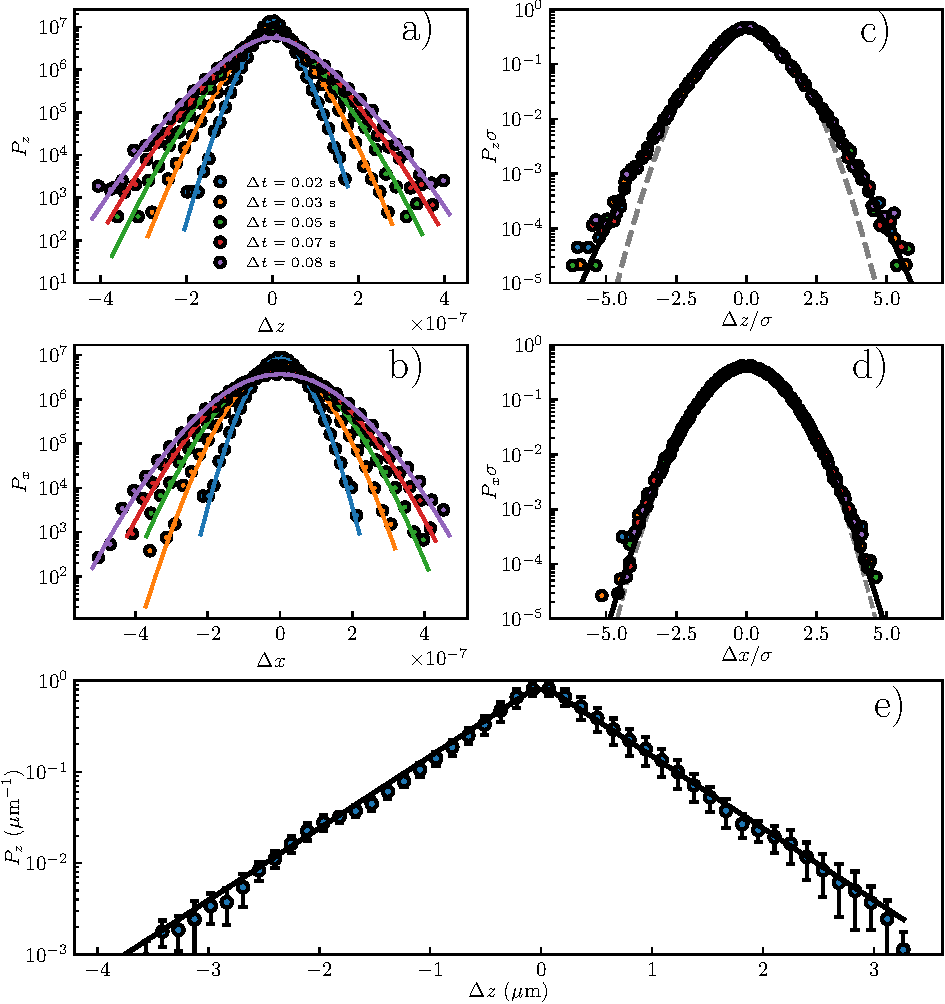
\includegraphics{02_body/chapter3/images/trajctory_analysis/P_displacement.pdf}
	\caption{a, b) Probability density functions $P_i$ of the displacements $\Delta x$ and $\Delta z$, at short times. The solid lines are the best fits to Eq.~(\ref{Eq:PDzshort}), using Eqs.~(\ref{Eq:PDF}),~(\ref{Eq:etaz}),~and~(\ref{Eq:etax}), with $B = 4.8$, $\ell_\mathrm{D} = 21 ~ \mathrm{nm}$, and $\ell_\mathrm{B} = 530~\mathrm{nm}$. c,d) Normalized probability density functions $P_i\,\sigma$ of the normalized displacements $\Delta x/\sigma$ and $\Delta z/\sigma$, at short times, with $\sigma^2$ the corresponding MSD (see panel Fig.~\ref{fig.MSD}), for different time increments $\Delta t$ ranging from 0.0167~s to 0.083~s, as indicated with different colors. The solid lines are the best fits to Eq.~(\ref{Eq:PDzshort}), using Eqs.~(\ref{Eq:PDF}),~(\ref{Eq:etaz}),~and~(\ref{Eq:etax}), with $B = 4.8$, $\ell_\mathrm{D} = 21 ~ \mathrm{nm}$, and $\ell_\mathrm{B} = 530~\mathrm{nm}$. For comparison, the gray dashed lines are normalized Gaussian distributions, with zero means and unit variances. d) Probability density function $P_z$ of the displacement $\Delta z$, at long times, averaged over several values of $\Delta t$ ranging between 25 s and 30~s. The solid line is the best fit to Eq.~(\ref{auxiliary}), using Eq.~(\ref{Eq:PDF}), with $B = 4.8$, $\ell_\mathrm{D} = 21 ~ \mathrm{nm}$, and $\ell_\mathrm{B} = 530~\mathrm{nm}$.}
	\label{fig.displacement}
\end{figure}



\subsubsection{Local diffusion coefficient inference}

We now wish to go beyond the previous average $\langle D_i\rangle$ of Eq.~(\ref{averagediff}), and resolve the local diffusion coefficient $D_i(z)$. To measure local viscosity from experimental trajectories, a binning method is generally employed~\cite{friedrich_approaching_2011}. This method consists of constructing the displacement \gls{PDF} conditioned on the particle height, a measure the distribution's variance $\sigma_i(z_0) = \sqrt{2D_i (z_0) \Delta t}$ as in Eq.~(\ref{Pdxshort}). 


\begin{figure}[h!]
	\centering
	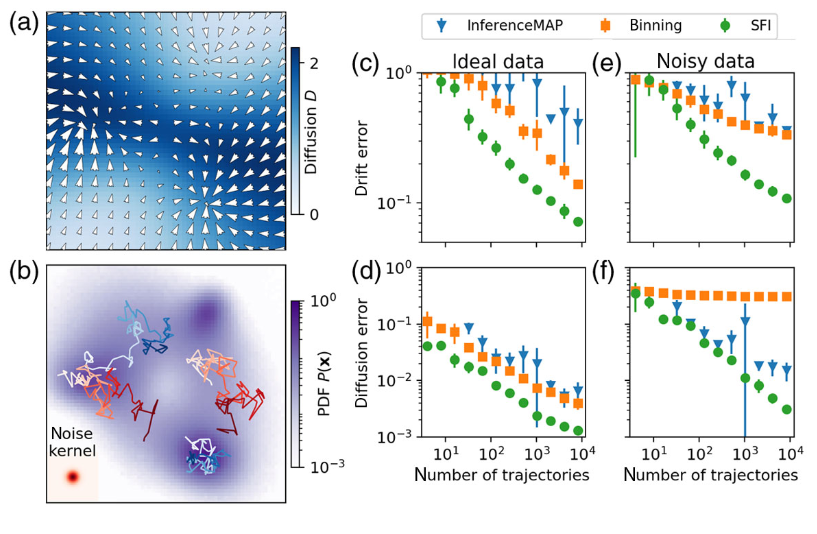
\includegraphics[scale=0.6]{02_body/chapter3/images/diffusion_coefficient/figure_Ronceray.png}
	\caption{Figure from \cite{frishman_learning_2020}. Quantitative comparison of Surface Force Inference (\gls{SFI} with other methods on a simulated system mimicking 2D single-molecule trajectories in a complex environment with space-dependent isotropic diffusion. a) The diffusion field (blue gradient) and drift field (white arrows). b) The steady-state distribution function (\gls{PDF}) of the process. The traces are representative trajectories of $100$ time steps. c-f) Comparison of the performance of \gls{SFI} and two widely used inference methods: InferenceMAP, a method for single-molecule inference (blue triangles)  \cite{beheiry_inferencemap_2015}, and grid-based binning with maximum-likelihood estimation \cite{hoze_heterogeneity_2012, friedrich_approaching_2011} (orange squares). They evaluated the performance of these methods on the approximation of the drift field (c),e)) and diffusion field (d)f)) as a function of the number $N$ of single-molecule trajectories (similar to the ones in panel b)) used. With ideal data (c),d)) and in the presence of measurement noise(e),f)). The performance is evaluated as the average mean-squared error on the reconstructed field along trajectories. \gls{SFI} outperforms both other methods in all cases. More information about the parameters of their simulation and analysis can be found in their work \cite{frishman_learning_2020}.}
	\label{fig.ronceray}
\end{figure}

Although the binning method is well suited for drift measurements, it suffers from a lack of convergence and precision when second moments or local diffusion coefficients have to be extracted. In particular, the binning method did not allow us to measure specifically the local diffusion coefficient in the key interfacial region corresponding to $z<100$~nm. Indeed, as we can observe in the Fig.~\ref{fig.ronceray}-f) the diffusion error on noisy (such as experimental) data does saturate of the binning method is outperformed by a robust developed method  recently developed by Frishman and Ronceray \cite{frishman_learning_2020}. This method uses Stochastic Force Inference (\gls{SFI}), in order to evaluate spatially varying force fields and diffusion coefficients, from the information contained within the trajectories. 

In practice \gls{SFI} can reconstruct force and diffusion fields and measure entropy production from Brownian trajectories. \gls{SFI} is based on the communication-theory notion of capacity which is an information-theoretic bound, when the system is viewed as a communication channel, that limit at which rate information about the fields can be extracted from a Brownian trajectory. To explain the method, let us consider a Brownian particle that obey to the equation similar to Eq.~(\ref{Eq.langevin_confined}), using $\mu$ to denotes the $x$-, $y$- and $z$-axis:

\begin{equation}
	\dot{x}_\mu = F_\mu (x) + \partial_\nu D(x)_{\mu \nu} + \sqrt{2D(x)}_{\mu \nu} \textnormal{d}B_t~,
\end{equation}

where the Einstein summation is used over repeated indices, and the force field $F_\mu (x)$ and the diffusion tensor $D_{\mu \nu}$ are assumed to be time-independent. This method is built to measure the entire diffusion matrix, which for a particle diffusing above a wall has non-zero the diagonal term (\textit{i.e.} $D_{xx}$, $D_{yy}$ and $D_{zz}$). However, for more complex environment such as cellular environment as shown on Fig.~\ref{fig.ronceray}-a), non-diagonal terms exist leading to correlations between the displacement axis. As an example, it has been observed in elastohydrodynamics \cite{saintyves_self-sustained_2016} that the parallel movement near a soft wall can induce perpendicular forces, hence leading in that peculiar case, to correlation between the $x$ and $z$ movement. The \gls{SFI} idea is to approximate the diffusion field as a linear combination of a basis of $n_b$ known functions $b={b_\alpha (x)}_{\alpha = 1,...,n_b}$. For the diffusion of spherical spheres near a wall where the diffusion coefficient is given by the Eqs.~(\ref{Eq:etaz})~and~(\ref{Eq:etax}) we got robust results using their built-in polynomial basis:

\begin{equation}
	b = \{b_\alpha (x)\}_{\alpha= 1,...,n_b} = \{1, x_\mu, x_\mu x_\nu, ...\} \text{ (up to the order } n_b \text{ )}.
\end{equation} 

They perform this approximation by projecting the diffusion field onto the space spanned by $b_\alpha (x)$ using the position \gls{PDF}, $P_\mathrm{eq}$ (see Eq.~(\ref{Eq:PDF})) as a measure. This corresponds to a least-squares fit of the diffusion field by linear combinations of the $b_\alpha$'s. To do this fit, they define a projector:

\begin{equation}
	c_\alpha (x) = B^{1/2}_{\alpha \beta} b_\beta (x) ~,
\end{equation}

where $ B^{1/2}_{\alpha \beta}$ is an orthonormalization matrix such that $\int c_\alpha c_\beta P_\mathrm{eq}(x)\mathrm{d}x = \delta _{\alpha \beta}$. They then approximate $D_{\mu \nu}$ by its projection as a linear combination of known functions:

\begin{equation}
	D_{\mu \nu} (x) \simeq D_{\mu \nu \alpha} c_\alpha (x) ~,
\end{equation}  

with,

\begin{equation}
	D_{\mu \nu \alpha} = \int D_{\mu \nu}(x) c_\alpha (x) P_\mathrm{eq} \mathrm{d}x ~.
\end{equation}

As the equation here are over a whole trajectory which is long enough to satisfy $P_\mathrm{eq}$, the empirical projector $\hat{c}_\alpha$ can be approximated using the trajectory averages. To measure the local diffusion they construct a local estimator $\hat{d}_{\mu \nu} = \Delta x_\mu (t_i) \Delta x_\nu (t_i) / 2\Delta t$, so that $D_{\mu \nu \alpha}$ now reads:

\begin{equation}
	\hat{D}_{\mu \nu \alpha} = \frac{1}{\tau} \sum _i \hat{d}_{\mu \nu} (t_i) \hat{c}_\alpha (x (t_i)) \Delta t).
\end{equation}

The latter equation corresponds to a linear regression of $\hat{d}_{\mu \nu} (t_i)$, and permits to project the diffusion tensor onto a finite set of basis functions. We implemented this method, using fourth-order polynomials in our case. to simplify the use of their method with our data, I developed a simple Python function around their method \href{https://github.com/eXpensia/StochasticForceInference/blob/master/fun_SFI.py}{\faGithub} which can infer the local diffusion coefficient by only one function call: 

\begin{minted}
	[
	frame=lines,
	framesep=2mm,
	baselinestretch=1.2,
	fontsize=\footnotesize,
	linenos
	]{text}


Dx, Dy, Dz, z_D = Compute_diffusion(pos)

\end{minted}

Where in the latter \mintinline{python}{pos}, is the 3D trajectory of a Brownian colloid. It allowed us to infer the local diffusion coefficients $D_i(z)$, down to $z=10$~nm, as shown in Fig.~\ref{fig.visco}. The results are in excellent agreement with the theoretical predictions, $D_{\parallel}(z)$ and $D_z(z)$, using  Eqs.~(\ref{Eq:etaz})~and~(\ref{Eq:etaz}), thus validating the method.


\begin{figure}[H]
	\centering
	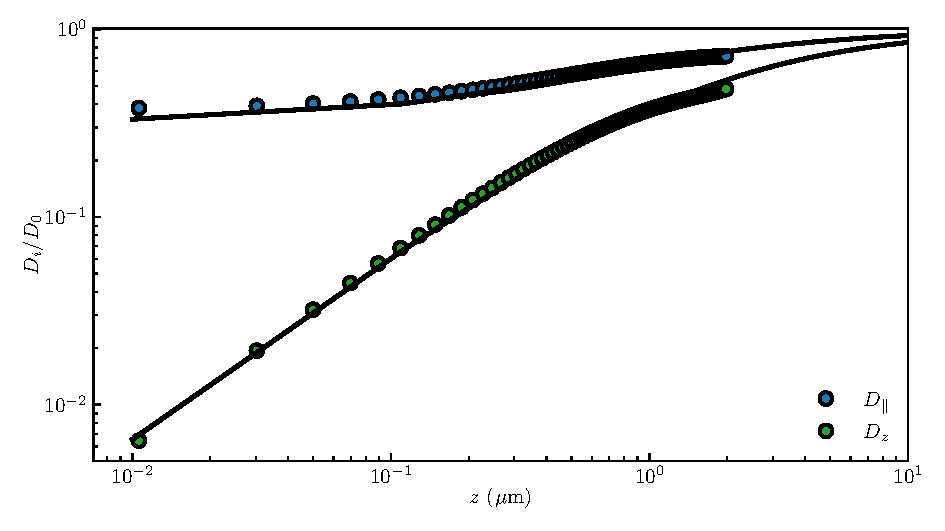
\includegraphics{02_body/chapter3/images/trajctory_analysis/visco.pdf}
	\caption{ Measured local short-term diffusion coefficients $D_i$ of the microparticle, normalized by the bulk value $D_0$, as functions of the distance $z$ to the wall, along both a transverse direction $x$ or $y$ ($D_i=D_\parallel=D_x=D_y$, blue) and the normal direction $z$ ($D_i=D_z$, green) to the wall. The solid lines are the theoretical predictions, $D_{\parallel}(z)=D_0\eta/\eta_{\parallel}(z)$ and $D_z(z)=D_0\eta/\eta_z(z)$, using the local effective viscosities $\eta_{\bot}(z)$ and $\eta_\parallel(z)$ of Eqs.~(\ref{Eq:etaz})~and~(\ref{Eq:etaz}), respectively.}
	\label{fig.visco}
\end{figure}

\subsubsection{Precise potential inference using multi-fitting technique}
So far, through Figs.\ref{fig.pdf_exp} to \ref{fig.visco}, we have successively presented the various measured statistical quantities of interest, as well as their fits to corresponding theoretical models. Therein, we have essentially three free physical parameters, $B$, $\ell_\mathrm{B}$, $\ell_\mathrm{D}$, describing the particle and its environment, as well as the \textit{a priori} undetermined location of the $z=0$ origin. These four parameters are actually redundant among the various theoretical models. Therefore, in order to measure them accurately, we in fact perform all the fits simultaneously,
using a Broyden-Fletcher-Goldfarb-Shanno (BFGS) algorithm that is well suited for unconstrained
nonlinear optimization~\cite{dai_convergence_2002}. To do so, we construct a global minimizer:
\begin{equation}
	\chi ^ 2 = \sum _{n=1} ^{N} \chi_n ^ 2\ ,
\end{equation}
where we introduce the minimizer $\chi _n ^2$ of each set $n$ among the $N$ sets of data, defined as:
\begin{equation}
	\chi _n ^2 = \sum _{i=1} ^{M_n} \frac{[y_{ni} - f_n(x_{ni}, \mathbf{b})]^2 }{f_n(x_{ni}\ , \mathbf{b})^2}\ ,
\end{equation}
with $\{x_{ni},y_{ni}\}$ the experimental data of set $n$, $M_n$ the number of experimental data points for set $n$, $f_n$ the model for set $n$, and $\mathbf{b}=(b_1,b_2,...,b_p)$ the $p$ free parameters. In our case, $p=4$, and $\{x_{ni},y_{ni}\}$ represent all the experimental data shown in Figs.\ref{fig.pdf_exp} to \ref{fig.visco}. 

Due to strong dependence of the normal diffusion coefficient $D_z$ with $z$, it is possible to find the wall position with a 10 nm resolution, thus overcoming a drawback of the Lorenz-Mie technique which only provides the axial distance relative to the focus of the objective lens. Besides, the three physical parameters globally extracted from the multifitting procedure are: $B = 4.8 \pm 0.6$, $\ell_\mathrm{D} = 21 \pm 1~ \mathrm{nm} $, and $\ell_\mathrm{B} = 530 \pm 2~ \mathrm{nm}$. Using the particle radius $a = 1.518 \pm 0.006 ~ \mathrm{\mu m}$ calibrated from the preliminary fits of the interference patterns to the Lorenz-Mie scattering function (see section \ref{sec:radius_charac}), and the $1050 ~ \mathrm{kg.m^{-3}}$ tabulated bulk density of polystyrene, we would have expected $\ell_\mathrm{B}=559 ~ \mathrm{nm}$ instead, which corresponds to less than $2\,\%$ error, and might be attributed to nanometric offsets, such as \textit{e.g.} the particle and/or wall rugosity. 

\subsubsection{Measuring external forces using the local drifts}
Finally, we investigate the total conservative force $F_z(z)$ acting on the particle along $z$. The first method way to measure it is to calculate the gradient of the potential $U$ which is experimentally measured from the position \gls{PDF} giving:


\begin{equation}
	F_z^\mathrm{eq} = -\nabla U = k_\mathrm{B}T \frac{\partial}{\partial z} \ln (P_\mathrm{eq}) ~,
	\label{Eq.conservative_force}
\end{equation}

where one can use the experimentally measured $P_\mathrm{eq}$ (see Fig.~\ref{fig.pdf_exp}) the results of this method is shown in fig.\ref{fig.figure_force_total}. However, it can be interesting to measure the forces using the local drifts as for more complex systems, some non-conservative forces could arise. As the Eq.~(\ref{Eq.conservative_force}) only take into account to the potential $U$, only conservative forces can be extracted from the measurement of $P_\mathrm{eq}$. For more complex system, non-conservative forces could be measured by the difference between forces obtained through $P_\mathrm{eq}$ and the local drifts.  By averaging the overdamped Langevin equation over a fine-enough $z$-binning grid and short enough time interval $\Delta t$, one gets in the Itô convention (corresponding to our definition of $\Delta z$):
\begin{equation}
	F_z (z) = 6 \pi \eta_z (z ) a \frac{\langle\Delta z\rangle}{\Delta t} - k_\mathrm{B}T \frac{D_z'(z)}{D_z(z)} \ ,
	\label{stokes}
\end{equation}
where the last term corresponds to the additional contribution due to the non-trivial integration of the multiplicative noise~\cite{volpe_influence_2010,mannella_comment_2011,mannella_ito_2012, sancho_brownian_2011}, with the prime denoting the derivative with respect to $z$. From the averaged measured vertical drifts $\langle\Delta z\rangle$, and invoking Eq.~(\ref{Eq:etaz_pade}), one can reconstruct $F_z(z)$ from Eq.~(\ref{stokes}), as shown in Fig.~\ref{fig.figure_force_total}. We stress that the statistical error on the force measurement is comparable to the thermal-noise limit~\cite{liu_subfemtonewton_2016}: 
\begin{equation}
	\label{tnl}
	\Delta F=\sqrt{24\pi k_{\mathrm{B}}T \eta_z(z) a/ \tau_{\textrm{box}}(z)}\ ,
\end{equation}
where $\tau_{\textrm{box}}(z)$ is the total time spent by the particle in the corresponding box of the $z$-binning grid. To corroborate these measurements, we invoke Eq.~(\ref{Eq:PDF}) and express the total conservative force $F_z(z)=-U'(z)$ acting on the particle along $z$:
\begin{equation}
	\displaystyle F_z(z) =  k_{\mathrm{B}}T\left(\frac{B}{\ell_\mathrm{D}} \textrm{e}^{-\frac{z}{\ell_\mathrm{D}}} - \frac{1}{\ell_\mathrm{B}}\right)\ .
	\label{Eq:Force}
\end{equation} 
Using the physical parameters extracted from the above multifitting procedure, we plot Eq.~(\ref{Eq:Force}) in Fig.~\ref{fig.figure_force_total}. The agreement with the data is excellent, thus showing the robustness of the force measurement. In particular, we can measure forces down to a distance of $40$~nm from the surface. Besides, far from the wall, we are able to resolve the actual buoyant weight $F_{\textrm{g}} =- 7  \pm 4 ~ \mathrm{fN}$ of the particle. This demonstrates that we reach the femtoNewton resolution, and that this resolution is solely limited by thermal noise.
\begin{figure}[H]
	\centering
	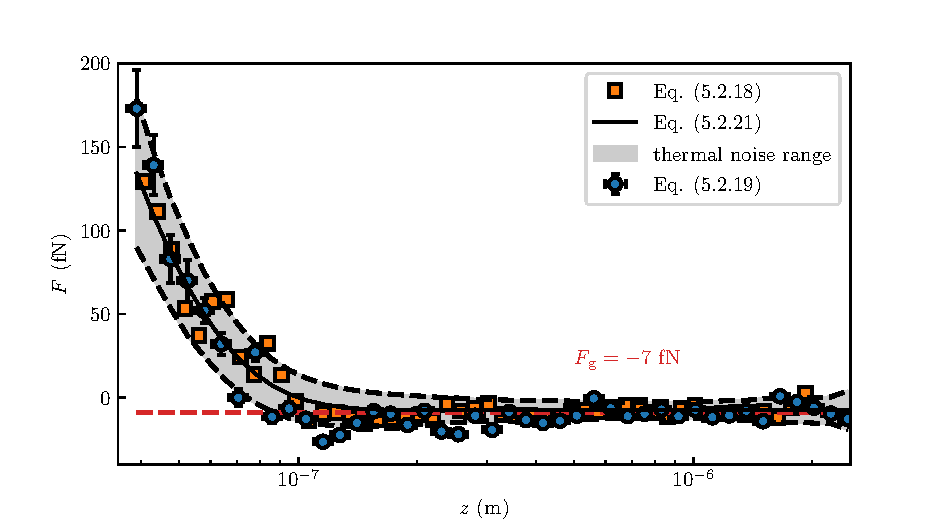
\includegraphics{02_body/chapter3/images/trajctory_analysis/figure_force_total.pdf}
	\caption{Total normal conservative force $F_z$ exerted on the particle as a function of the distance $z$ to the wall, reconstructed from Eq.~(\ref{stokes}), using Eq.~(\ref{Eq:etaz_pade}) in circles and using Eq.~(\ref{Eq.conservative_force}) in squares. The solid line corresponds to Eq.~(\ref{Eq:Force}), with $B=4.8$, $\ell_{\mathrm{D}}=21\,\mathrm{nm}$ and $\ell_{\mathrm{B}}=530\,\mathrm{nm}$. The black dashed lines and gray area indicate the amplitude of the thermal noise computed from Eq.~(\ref{tnl}). The horizontal red dashed line indicates the buoyant weight $F_{\textrm{g}}=-7$~fN of the particle.}
	\label{fig.figure_force_total}
\end{figure}

\subsection{Conclusion}
To conclude, we have successfully built a multi-scale statistical analysis for the problem of freely diffusing individual colloids near a rigid wall. Combining the equilibrium distribution in position, time-dependent non-Gaussian statistics for the spatial displacements, a novel method to infer local diffusion coefficients, and a multifitting procedure, allowed us to reduce drastically the measurement uncertainties and reach the nanoscale and thermal-noise-limited femtoNewton spatial and force resolutions, respectively. The ability to measure tiny surface forces, locally, and at equilibrium, as well the possible extension of the method to non-conservative forces and out-of-equilibrium settings~\cite{amarouchene_nonequilibrium_2019, mangeat_role_2019}, opens fascinating perspectives for nanophysics and biophysics.

